%%	SECCION documentclass																									 %%	
%%---------------------------------------------------------------------------%%
\documentclass{article}

%%---------------------------------------------------------------------------%%
%%	SECCION usepackage																											 %%	
%%---------------------------------------------------------------------------%%
\usepackage{amsmath, amsthm}
\usepackage[spanish,activeacute]{babel}
\usepackage{caratula}
\usepackage{a4wide}
\usepackage{hyperref}
\usepackage{fancyhdr}
% \usepackage{moreverb}
\usepackage{graphicx} % Para el logo magico!
\usepackage{capt-of}
\usepackage{afterpage}
\usepackage{float}
\usepackage{amssymb}
\usepackage{amsmath}
\usepackage[latin1]{inputenc}
\usepackage{subfigure}
\usepackage{algorithm}
\usepackage{algorithmic}
\usepackage[dvipsnames,usenames]{color}
\usepackage{amsfonts}
\usepackage{code_color}
\usepackage{amsthm}
\usepackage{marvosym}
%\usepackage{minipage}

%%---------------------------------------------------------------------------%%
%%	SECCION opciones																												 %%	
%%---------------------------------------------------------------------------%%
\parskip    = 11 pt
\headheight	= 13.1pt
\pagestyle	{fancy}
\definecolor{orange}{rgb}{1,0.5,0}

\addtolength{\headwidth}{1.0in}

\addtolength{\oddsidemargin}{-0.5in}
\addtolength{\textwidth}{1.0in}
\addtolength{\topmargin}{-0.8in}
\addtolength{\textheight}{0.7in}

%%%---------------------------------------------------------------------------%%
%%%	SECCION listings    													 %%	
%%%---------------------------------------------------------------------------%%
%\usepackage{listings}
%\lstset{
%		language=C++,
%		basicstyle=\ttfamily \small,
%		keepspaces=true,
%		flexiblecolumns=false,
%		basewidth={0.5em,0.45em},
%		keywordstyle=\ttfamily \bfseries \hlkwa,
%		tabsize=4
%}

%%---------------------------------------------------------------------------%%
%%	SECCION document	 %%	
%%---------------------------------------------------------------------------%%
\begin{document}
\renewcommand{\chaptername}{Parte }
\renewcommand{\algorithmicrequire}{\textcolor{blue}{\textbf{Requiere:}}}
\renewcommand{\algorithmicensure}{\textbf{Devuelve:}}
\renewcommand{\algorithmicend}{\textbf{Fin}}
\renewcommand{\algorithmicif}{\textcolor{blue}{\textbf{Si}}}
\renewcommand{\algorithmicthen}{\textcolor{blue}{}} %%\textbf{entonces}}}
\renewcommand{\algorithmicelse}{\textcolor{red}{\textbf{Si no}}}
\renewcommand{\algorithmicelsif }{\textcolor{blue}{\textbf{Si no y}}}
\renewcommand{\algorithmicendif}{\textcolor{blue}{\textbf{Fin si}}}
\renewcommand{\algorithmicfor}{\textcolor{ForestGreen}{\textbf{Para}}}
\renewcommand{\algorithmicendfor}{\textcolor{ForestGreen}{\textbf{Fin para}}}
\renewcommand{\algorithmicwhile}{\textcolor{ForestGreen}{\textbf{Mientras}}}
\renewcommand{\algorithmicendwhile}{\textcolor{ForestGreen}{\textbf{Fin mientras}}}
\renewcommand{\algorithmicdo}{\textcolor{ForestGreen}{}} %%\textbf{hacer}}}
\renewcommand{\algorithmicreturn}{\textbf{Devolver}}
\floatname{algorithm}{Algoritmo}

%%---- Caratula -------------------------------------------------------------%%
\materia{Problemas, algoritmos y programaci�n (2010)}
\titulo{Trabajo Pr'actico n� 2}


\integrante{Barenbaum, Pablo}{124/04}{foones@gmail.com}
\integrante{Mart'inez, Federico}{17/06}{federicoemartinez@gmail.com}
\integrante{Sainz-Tr'apaga, Gonzalo}{454/06}{gonzalo@sainztrapaga.com.ar}
\grupo{Grupo 1}
\resumen{
El siguiente informe presenta la resoluci�n a los 4 problemas correspondientes al segundo trabajo pr\'actico de la materia problemas, algoritmos y programaci�n en el primer cuatrimestre del 2010. En el mismo se encuentra la explicaci�n del algoritmo utilizado para resolver cada problema, as� como tambi�n la implementaci�n en C++ de los mismos.
}

% TOC, usa estilos locos
\maketitle
\pagestyle{empty}
{
\fancypagestyle{plain}
    {
    \fancyhead{}
    \fancyfoot{}
    \renewcommand{\headrulewidth}{0.0pt}
    } % clear header and footer of plain page because of ToC
%\tableofcontents
}

\newpage
% arreglos los estilos para el resto del documento, y
% reseteo los numeros de pagina para que queden bien
\pagenumbering{arabic}
\fancypagestyle{plain} {
    \fancyhead[LO]{Barenbaum, Mart�nez, Sainz Tr�paga}
    \fancyhead[C]{}
    \fancyhead[RO]{P\'agina \thepage\ de \pageref{LastPage}}
    \fancyfoot{}
    \renewcommand{\headrulewidth}{0.4pt}
}
\pagestyle{plain}
\section{10362 - Trains}
\textbf{Problema:} Dado un conjunto de rutas de tren, determinar las conexiones
``\'optimas'' entre dos estaciones dadas. Una conexi\'on $c$ es \'optima
si se cumple lo siguiente:

\begin{enumerate}
\item[(A)] No hay una conexi\'on $c'$ que salga m\'as tarde y llegue m\'as temprano o a la misma hora que $c$.
\item[(B)] No hay una conexi\'on $c'$ que salga a la misma hora y llegue m\'as temprano que $c$.
\end{enumerate}

\subsection{Resoluci�n}

La idea del algoritmo propuesto es primero encontrar los caminos m\'as
cortos (en minutos) entre la estaci\'on de origen y la estaci\'on de
destino. Estos cumplen con la condici\'on (B). Una vez hecho esto,
determinar cu\'ales de ellos cumplen con la condici\'on (A).

El problema de encontrar los caminos m\'as cortos se modela como un
problema de camino m\'inimo.

\subsubsection{Descripci\'on del grafo asociado al problema}
En primer lugar, construimos un grafo orientado con pesos en los ejes
$G = (V,E)$, cuyos nodos
representan una estaci\'on y una hora del d\'ia, y cuyos ejes representan
una manera de llegar de una pareja estaci\'on/hora a otra. El grafo
contiene los siguientes nodos:

$(n,h)\in V \longleftrightarrow$ existe un tren que pasa por la estaci\'on
$n$ a las $h$ horas $(h \in [\text{0:00}..\text{23:59}])$

%%$FINAL \in V$

Adem\'as, hay un eje desde $(n_1,h_1)$ hasta $(n_2,h_2) \longleftrightarrow$ se cumple alguno de los dos casos siguientes:
\begin{enumerate}
\item Existe un tren que pasa por $n_1$ a las $h_1$ y cuya siguiente parada es en $n_2$ a las $h_2$ (sin pasar por estaciones intermedias).
\item $n_1 = n_2$ (es la misma estaci\'on) y $h_2$ es el horario que sigue a $h_1$ en orden cronol\'ogico, sin pasar por horas intermedias.
\end{enumerate}
%\begin{enumerate}
%\item existe una ruta que permite tomar un tren en $n_1$ a las $h_1$ y llegar a $n_2$ a las $h_2$.
%\item $n_1=n_2 \wedge h_1<h_2 \wedge \nexists h_3 / (n_1,h_3) \in V \wedge h_1 < h_3 < h_2$
%\item $n_1=n_2 \wedge h_1 > h_2 \wedge \nexists h_3 / (n_1,h_3) \in V \wedge ( h_1 < h_3 \vee h_3 < h_2)$
%\end{enumerate}

Los ejes que resultan de la primera condici\'on tienen como peso asociado el tiempo de viaje.
Si bien se conoce la hora del d\'ia asociada a cada nodo, es necesario conocer el peso
expl\'icitamente, porque el tiempo de viaje entre dos estaciones {\em puede} ser mayor a un d\'ia.

Los ejes que resultan de la segunda condici\'on representan la posibilidad de quedarse
en una estaci\'on y esperar el pr�ximo tren. En este caso, el peso del eje es la diferencia
entre $h_2$ y $h_1$. Cuando decimos que $h_2$ es el horario que sigue a $h_1$
``en orden cronol\'ogico'', tambi\'en hay que considerar que $h_1$ puede ser
el \'ultimo tren del d\'ia y $h_2$ el primer tren del d\'ia siguiente. En ese caso
el peso del eje es la diferencia m\'odulo 24 horas.

%TODO: esto hay que explicarlo mas y/o mejor?
El grafo descripto modela el problema porque una conexi�n permite
llegar de una estaci\'on/hora a otra si y s\'olo si existe
un camino entre los dos nodos correspondientes del grafo, de manera tal que el tiempo que
tarda la conexi\'on es el peso del camino. Esto es porque o bien el
camino es una ruta directa sin cambiar de tren (en cuyo caso, por
los ejes del caso $1$, hay un camino en el grafo con el peso apropiado),
o bien la conexi�n usa fragmentos de varias rutas. Para hacer esto,
es necesario esperar cierto tiempo en una estaci\'on para cambiar de tren.
El tiempo de espera debe ser contabilizado
tambi�n, lo que se logra con los ejes del caso $2$. Si es posible hacer
una combinaci�n sin esperar, es porque se llega a una estaci\'on a la misma
hora en que sale el siguiente tren. Esto no representa un problema
porque el enunciado indica que el tiempo necesario para realizar la conexi�n
est� incorporado en los horarios de los trenes. Por el caso $1$, ese nodo
tiene ambos ejes, y el camino es realizable. De manera similar
se ve lo inverso, es decir que cualquier camino en el grafo representa
una conexi\'on v\'alida.

Notar que, en el primer caso, se agrega un eje s\'olo cuando la ruta no pasa por estaciones
intermedias. De manera similar, en el segundo caso, se agrega un eje de $(n,h_1)$ a $(n,h_2)$
s\'olo cuando no existe un horario $h_3$ entre $h_1$ y $h_2$.
Es decir, el grafo se construye {\em sin} hacer la clausura transitiva
de los ejes. No es necesario agregar los ejes restantes, porque lo que
importa es la duraci\'on en minutos de los caminos, y todos
los caminos posibles est\'an dados precisamente la clausura transitiva
de los ejes.
La ventaja es que de esta manera la cantidad de ejes del grafo
es lineal en el tama\~no de la entrada.

\subsubsection{B\'usqueda de los caminos m\'inimos}

Una vez que se tiene el grafo descripto en la secci\'on anterior,
el objetivo es determinar las duraciones de las conexiones \'optimas.
Las conexiones \'optimas deben ser caminos m�nimos entre nodos de la estaci\'on de origen
($src$) y la estaci\'on de destino ($dst$). Si no se tratara de caminos m�nimos, ser�a posible
encontrar un camino que sale a la misma hora y llega antes (de menor duraci\'on, y por
lo tanto de menor peso), y la conexi�n no ser�a \'optima por no cumplir con
la condici\'on (B).

El primer objetivo es determinar, para cada nodo $(src,h)$ el peso del
camino m\'inimo hasta alg\'un nodo $(dst,h')$.
Los pesos de los ejes son todos positivos, por lo cual es relativamente
sencillo convertir este problema en un problema de camino m\'inimo
{\em single-source}, para as\'i poder aplicar el algoritmo de Dijkstra.

Para convertir el problema, se agrega un nodo $\textsc{final}$ y, para
cada nodo de la forma $(dst,h)$, un eje de peso 0 hacia el nodo $\textsc{final}$.
Por \'ultimo, se considera el grafo $G'$ que resulta de invertir
todos los ejes en $G$ y se calculan los caminos m\'inimos en $G'$ desde
$\textsc{final}$ hasta todos los dem\'as nodos, usando el algoritmo
de Dijkstra.

Cada uno de los caminos m\'inimos encontrados en $G'$ que terminan en nodos
de la forma $(src,h)$, corresponden a alg\'un camino en $G$ que empieza en $(src,h)$,
llega hasta alg\'un nodo $(dst,h')$, y por \'ultimo llega a $\textsc{final}$
mediante un eje de peso 0. El peso del camino correspondiente en $G$ es m\'inimo
y es el mismo que el encontrado en $G'$.

%Por otro lado, todas los nodos cuya estaci\'on es la de destino, tienen un eje de costo $0$ con el nodo $FINAL$.

Como observaci\'on adicional, dado que lo que se busca son caminos
m\'inimos, si una estaci\'on $n$ tiene un \'unico horario $h$ en el que salen o
llegan trenes, durante la construcci\'on del grafo $G$ no se agrega el autoeje
$(n,h)$, porque este eje tiene peso de 24 horas y obviamente nunca es conveniente
(existe un camino desde $v$ hasta $w$ que pasa por dicho eje si y s\'olo si existe
un camino de $v$ a $w$ de menor peso que no lo utiliza).

\begin{figure}[H]
\centering
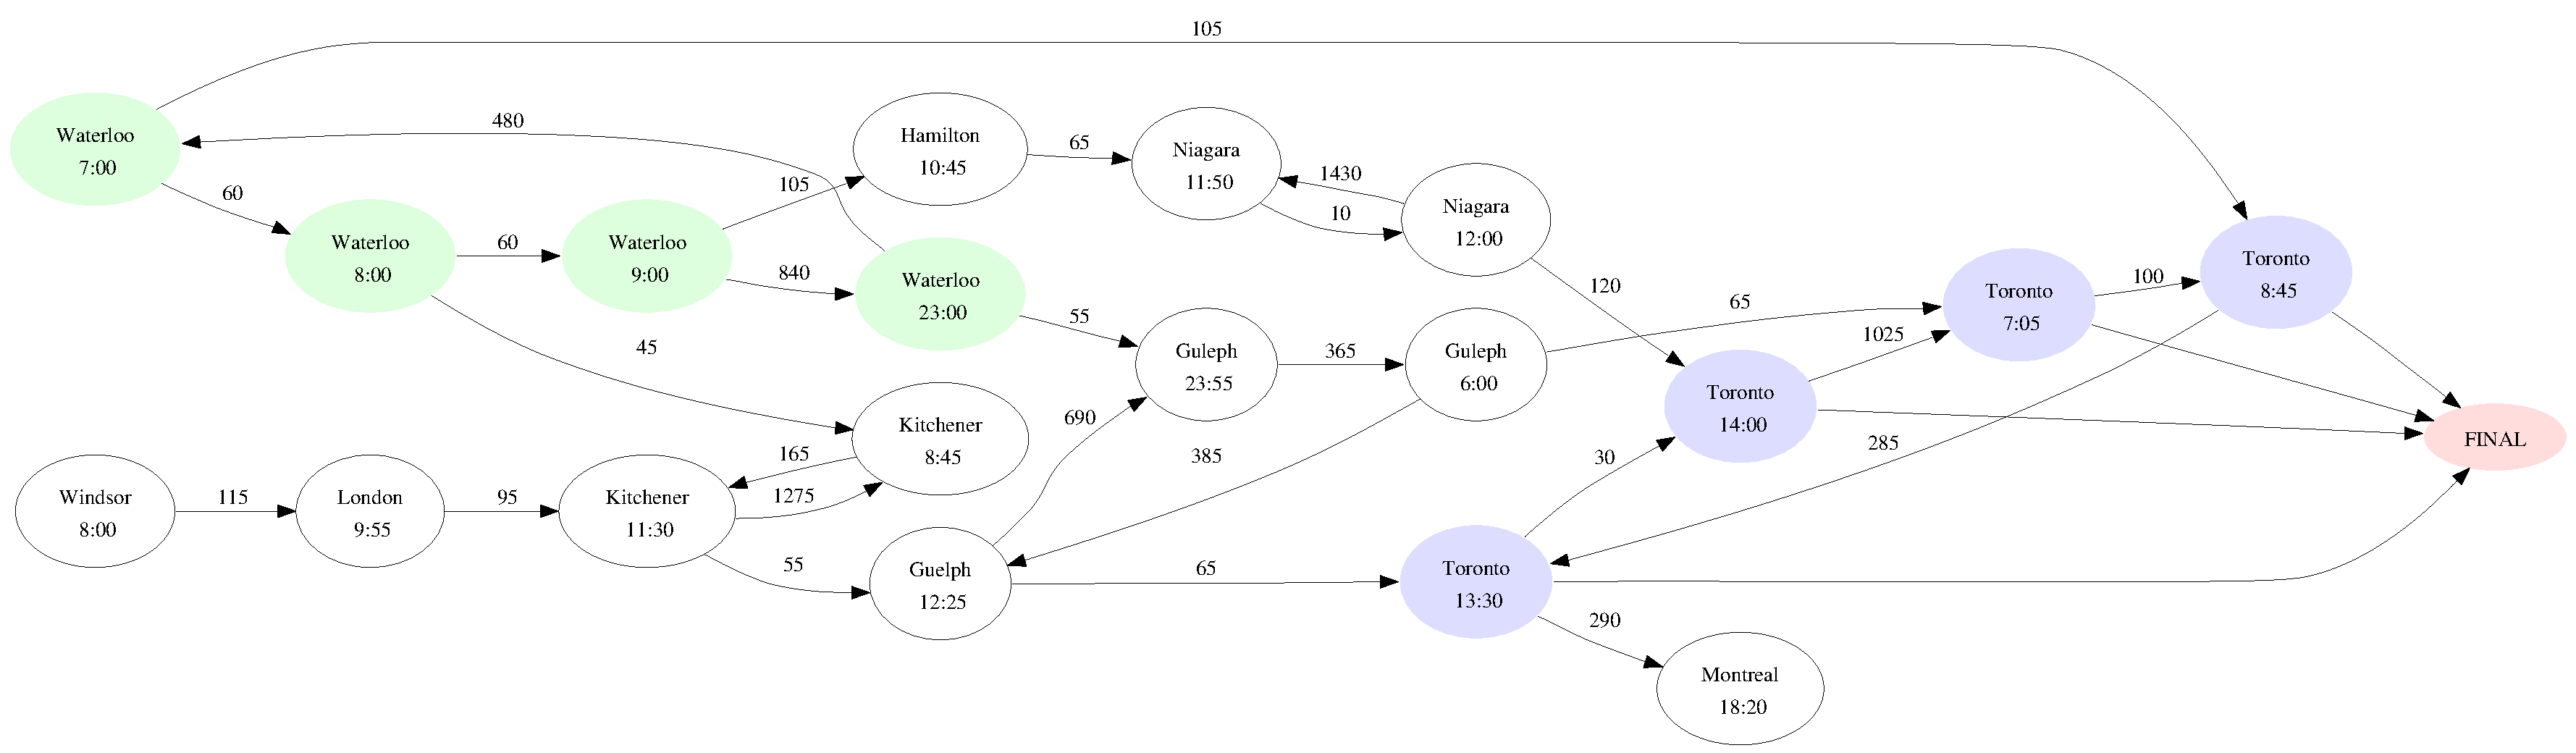
\includegraphics[scale=0.3]{./figuras/grafo.pdf}
\caption{Grafo resultante para la entrada de ejemplo (antes de invertir los ejes)}
\end{figure}

\subsubsection{Determinaci\'on de las conexiones \'optimas}

Una vez obtenidas las duraciones m\'inimas de los caminos que parten de cada
uno de los nodos $(src,h)$, resta s\'olo filtrar de esos caminos aquellos que
cumplen con la condici\'on (A).

Notar que la condici\'on (A) usa la expresi\'on ``llegar m\'as temprano'' en
el sentido que uno le atribuye intuitivamente, y no a la hora absoluta del d�a.
Por ejemplo, salir a las 21:00 y llegar a las 22:00 es llegar m\'as temprano
que salir a las 20:00 y llegar a la 1:00, pese a que $\text{1:00} < \text{22:00}$.
Esto es obvio, pero indica que la implementaci\'on debe comparar las duraciones
totales de los viajes m\'as que las horas de llegada.
Algo similar aplica para la expresi\'on ``salir m\'as tarde''.
%En la resoluci�n del problema consideramos el tiempo como cantidad de minutos.

El siguiente es el algoritmo para elegir las rutas, asumiendo que
las distancias desde cada nodo $v$ hasta el nodo $\textsc{final}$
ya fueron calculadas:

\begin{algorithm}[H]
\begin{algorithmic}
\caption{Determina las conexiones \'optimas}
\PARAMS{$distancia_v$ = duraci\'on m�nima de la conexi\'on desde un nodo $v$ hasta el nodo $\textsc{final}$}
\STATE m�nima hora de llegada $:= \infty$
\FOR{cada nodo $v$ de la forma $(src,h)$}
\STATE hora de llegada $:= h + distancia_{v} + $ 24 hs
\STATE\COMMENT{tiempo del nodo es la cantidad de tiempo hasta que sale el tren (i.e: si el tren sale a las 8, es la cantidad de minutos hasta las 8)}
\STATE m�nima hora de llegada $:= \min($hora de llegada, m�nima hora de llegada$)$
\ENDFOR 
\FOR{cada nodo $v$ de la forma $(src,h)$ (se recorren por hora decreciente)}
%\STATE hora de salida $:= h$
\STATE hora de llegada $:= h + distancia_{v}$
\IF{hora de llegada $<$ m�nima hora de llegada}
\STATE m�nima hora de llegada $:=$ hora de llegada
\STATE reportar la conexi\'on que sale a la hora $h$ y tarda $distancia_{v}$ en llegar
\ENDIF
\ENDFOR
\end{algorithmic}
\end{algorithm}

El primer {\bf for} inicializa el valor de la variable ``m\'inima hora de llegada''.
Para esto se busca, entre todos los nodos $(src,h)$, el que minimiza $h + distancia_{(src,h)} + \text{24 hs}$.
Este valor $H$ representa la hora m\'as temprana a la que se puede llegar a destino partiendo al
d\'ia siguiente, y se usa como cota superior para descartar algunas de las conexiones
que no son \'optimas.
Es decir, si $distancia_{(src,h)} \geq H$, la conexi\'on m\'as corta que empieza
en la estaci\'on de origen tomando el tren de la hora $h$ llega a lo sumo tan temprano
como alguna otra conexi\'on posterior, y por lo tanto no es \'optima.

Notar que alcanza con usar como cota superior la hora de llegada de
la conexi\'on m\'as corta que empieza en el {\em segundo} d\'ia
(y no es necesario mirar m\'as d\'ias hacia adelante) porque
la conexi\'on m\'as corta que empieza en el cualquier d\'ia
posterior al segundo llega despu\'es de $H$.

En el segundo {\bf for}, se tiene como invariante que la variable ``m\'inima hora de llegada''
es la m\'inima hora a la que se puede llegar con una conexi\'on que sale en
una hora posterior a $h$. Inicialmente esto es cierto porque, como ya se justific\'o,
``m\'inima hora de llegada'' se inicializa en $H$. El invariante se mantiene porque
los nodos se recorren por hora decreciente. En cada paso, si la hora a la que se
llega con una conexi\'on que empieza desde el nodo $v$ es menor que la m\'inima
hora a la que se puede llegar saliendo despu\'es de la hora $h$, esto quiere
decir que dicha conexi\'on cumple con la condici\'on (A). Adem\'as, es \'optima
porque tambi\'en cumpl\'ia con la condici\'on (B).

\subsubsection{Detalles de implementaci\'on y complejidad}

Todas las horas se representan en minutos. El grafo se representa con listas
de adyacencia. Cada nodo se identifica mediante un par $\langle id, hora \rangle$,
donde $id$ es un entero que representa una estaci\'on. Las listas de adyacencia se guardan
en un diccionario de nodo a lista de vecinos, cada uno con el peso del eje
correspondiente.

Llamamos $N$ a la cantidad de estaciones y $M$ a la cantidad de ejes
del grafo asociado al problema. Notar que $N \in O(M)$ porque no puede
haber nodos aislados, ya que si una estaci\'on
ocurre en la entrada, debe figurar en al menos una ruta. Adem\'as,
$M$ es lineal en el tama\~no de la entrada, porque
los ejes que representan el camino de un tren deben estar
expl\'icitos en la entrada, mientras la cantidad de ejes que
conectan nodos de la misma estaci\'on es (por la manera en la
que se construye el grafo) a lo sumo igual a la cantidad total
de nodos de la estaci\'on.
% Para construir el grafo, la informaci\'on de las estaciones
%se guarda en un diccionario que dado el nombre de la estaci\'on devuelve su
%id y el conjunto de horas a las que un tren pasa por dicha estaci\'on.

La implementaci\'on del algoritmo de Dijkstra usa una cola de prioridad
representada mediante un conjunto de tuplas $\langle distancia, nodo \rangle$,
por lo que la complejidad del algoritmo es $O(M \log N)$. El costo del
algoritmo que determina las conexiones \'optimas es $O(N \log N)$.
Previo a resolver el problema, el costo de procesar la entrada es el siguiente: 
\begin{itemize}
\item Primero se asigna un id a cada estaci\'on, y se construye un 
diccionario que permite ver, dada una estaci\'on (\texttt{string}), qu\'e
id tiene y a qu� horas hay trenes que llegan o salen. El costo de
esto es $O(N \log N)$ asumiendo, de acuerdo con el enunciado del
problema, que los nombres de las estaciones tienen un largo m\'aximo fijo
(y razonablemente chico).
\item Despu\'es se construyen las listas de adyacencia.
Esto toma $O(M \log N + N \log N)$. El segundo t�rmino proviene del costo de agregar 
los ejes entre nodos de la misma estaci�n. Esto se puede hacer en $O(N \log N)$ iterando las
claves del diccionario que guarda los ids y las horas de cada estaci\'on.
\end{itemize}

Finalmente la complejidad es $O(N \log N + M \log N) \subseteq O(M \log N)$.

\subsection{Implementaci�n}
\noindent
\ttfamily
\shorthandoff{"}\\
\hlstd{}\hlline{\ 1\ }\hldir{\#include\ $<$iostream$>$}\\
\hlline{\ 2\ }\hlstd{}\hldir{\#include\ $<$string$>$}\\
\hlline{\ 3\ }\hlstd{}\hldir{\#include\ $<$map$>$}\\
\hlline{\ 4\ }\hlstd{}\hldir{\#include\ $<$set$>$}\\
\hlline{\ 5\ }\hlstd{}\hldir{\#include\ $<$vector$>$}\\
\hlline{\ 6\ }\hlstd{}\hldir{\#include\ $<$list$>$}\\
\hlline{\ 7\ }\hlstd{}\hldir{\#include\ $<$cassert$>$}\\
\hlline{\ 8\ }\hlstd{}\hldir{\#include\ $<$cstdlib$>$}\\
\hlline{\ 9\ }\hlstd{}\\
\hlline{10\ }\hlkwa{using\ namespace\ }\hlstd{std}\hlsym{;}\\
\hlline{11\ }\hlstd{}\\
\hlline{12\ }\hldir{\#define\ forsn(i,\ s,\ n)\ for\ (int\ i\ =\ (s);\ i\ $<$\ (n);\ i++)}\\
\hlline{13\ }\hlstd{}\hldir{\#define\ forn(i,\ n)}\hlstd{\ \ }\hldir{forsn\ (i,\ 0,\ n)}\\
\hlline{14\ }\hlstd{}\hldir{\#define\ forall(x,\ s)\ for\ (typeof((s).begin())\ x\ =\ (s).begin();\ x\ !=\ (s).end();\ x++)}\\
\hlline{15\ }\hlstd{}\hldir{\#define\ dforall(x,\ s)\ for\ (typeof((s).rbegin())\ x\ =\ (s).rbegin();\ x\ !=\ (s).rend();\ x++)}\\
\hlline{16\ }\hlstd{}\\
\hlline{17\ }\hlkwc{typedef\ }\hlstd{}\hlkwb{int\ }\hlstd{Id}\hlsym{;\ }\hlstd{}\hlslc{//\ station\ id}\\
\hlline{18\ }\hlstd{}\hlkwc{typedef\ }\hlstd{}\hlkwb{int\ }\hlstd{Time}\hlsym{;}\\
\hlline{19\ }\hlstd{}\hlkwc{typedef\ }\hlstd{pair}\hlsym{$<$}\hlstd{Id}\hlsym{,\ }\hlstd{Time}\hlsym{$>$\ }\hlstd{Nodo}\hlsym{;}\\
\hlline{20\ }\hlstd{}\\
\hlline{21\ }\hlkwb{struct\ }\hlstd{Edge\ }\hlsym{\{}\\
\hlline{22\ }\hlstd{\ Nodo\ dest}\hlsym{;}\\
\hlline{23\ }\hlstd{\ Time\ cost}\hlsym{;}\\
\hlline{24\ }\hlstd{}\hlsym{\};}\\
\hlline{25\ }\hlstd{}\hlkwc{typedef\ }\hlstd{vector}\hlsym{$<$}\hlstd{Edge}\hlsym{$>$\ }\hlstd{Ady}\hlsym{;}\\
\hlline{26\ }\hlstd{}\hlkwc{typedef\ }\hlstd{map}\hlsym{$<$}\hlstd{Nodo}\hlsym{,\ }\hlstd{Ady}\hlsym{$>$\ }\hlstd{Grafo}\hlsym{;}\\
\hlline{27\ }\hlstd{}\\
\hlline{28\ }\hlkwc{typedef\ }\hlstd{map}\hlsym{$<$}\hlstd{string}\hlsym{,\ }\hlstd{pair}\hlsym{$<$}\hlstd{Id}\hlsym{,\ }\hlstd{set}\hlsym{$<$}\hlstd{Time}\hlsym{$>$\ $>$\ $>$\ }\hlstd{Stations}\hlsym{;}\\
\hlline{29\ }\hlstd{}\\
\hlline{30\ }\hlslc{//\ map$<$Nodo,\ Ady$>$::iterator}\\
\hlline{31\ }\hlstd{}\hldir{\#define\ \textunderscore nodo}\hlstd{\ \ }\hldir{first}\\
\hlline{32\ }\hlstd{}\hldir{\#define\ \textunderscore ady}\hlstd{\ \ }\hldir{second}\\
\hlline{33\ }\hlstd{}\\
\hlline{34\ }\hlslc{//\ Stations::iterator}\\
\hlline{35\ }\hlstd{}\hldir{\#define\ \textunderscore info}\hlstd{\ \ }\hldir{second}\\
\hlline{36\ }\hlstd{}\\
\hlline{37\ }\hlslc{//\ pair$<$Id,\ set$<$Time$>$\ $>$}\\
\hlline{38\ }\hlstd{}\hldir{\#define\ \textunderscore id}\hlstd{\ \ }\hldir{first}\\
\hlline{39\ }\hlstd{}\hldir{\#define\ \textunderscore timeset\ second}\\
\hlline{40\ }\hlstd{}\\
\hlline{41\ }\hlslc{//\ Nodo}\\
\hlline{42\ }\hlstd{}\hldir{\#define\ \textunderscore time}\hlstd{\ \ }\hldir{second}\\
\hlline{43\ }\hlstd{}\\
\hlline{44\ }\hldir{\#define\ HOUR\ 60}\\
\hlline{45\ }\hlstd{}\hldir{\#define\ DAY\ (24\ {*}\ HOUR)}\\
\hlline{46\ }\hlstd{\\
\hlline{47\ }Id\ }\hlkwc{inline\ }\hlstd{}\hlkwd{register\textunderscore station}\hlstd{}\hlsym{(}\hlstd{Stations}\hlsym{\&\ }\hlstd{stations}\hlsym{,\ }\hlstd{}\hlkwb{const\ }\hlstd{string}\hlsym{\&\ }\hlstd{station\textunderscore name}\hlsym{,\ }\hlstd{Time\ time}\hlsym{)\ \{}\\
\hlline{48\ }\hlstd{\ Stations}\hlsym{::}\hlstd{iterator\ }\hlkwd{it}\hlstd{}\hlsym{(}\hlstd{stations}\hlsym{.}\hlstd{}\hlkwd{find}\hlstd{}\hlsym{(}\hlstd{station\textunderscore name}\hlsym{));}\\
\hlline{49\ }\hlstd{\ }\hlkwa{if\ }\hlstd{}\hlsym{(}\hlstd{it\ }\hlsym{==\ }\hlstd{stations}\hlsym{.}\hlstd{}\hlkwd{end}\hlstd{}\hlsym{())\ \{}\\
\hlline{50\ }\hlstd{}\hlstd{\ \ }\hlstd{}\hlslc{//\ create}\\
\hlline{51\ }\hlstd{}\hlstd{\ \ }\hlstd{}\hlkwb{const\ }\hlstd{Id\ a\ }\hlsym{=\ }\hlstd{stations}\hlsym{.}\hlstd{}\hlkwd{size}\hlstd{}\hlsym{();}\\
\hlline{52\ }\hlstd{}\hlstd{\ \ }\hlstd{set}\hlsym{$<$}\hlstd{Time}\hlsym{$>$\ }\hlstd{s}\hlsym{;}\\
\hlline{53\ }\hlstd{}\hlstd{\ \ }\hlstd{s}\hlsym{.}\hlstd{}\hlkwd{insert}\hlstd{}\hlsym{(}\hlstd{time}\hlsym{);}\\
\hlline{54\ }\hlstd{}\hlstd{\ \ }\hlstd{stations}\hlsym{{[}}\hlstd{station\textunderscore name}\hlsym{{]}\ =\ }\hlstd{pair}\hlsym{$<$}\hlstd{Id}\hlsym{,\ }\hlstd{set}\hlsym{$<$}\hlstd{Time}\hlsym{$>$\ $>$(}\hlstd{a}\hlsym{,\ }\hlstd{s}\hlsym{);}\\
\hlline{55\ }\hlstd{}\hlstd{\ \ }\hlstd{}\hlkwa{return\ }\hlstd{a}\hlsym{;}\\
\hlline{56\ }\hlstd{\ }\hlsym{\}\ }\hlstd{}\hlkwa{else\ }\hlstd{}\hlsym{\{}\\
\hlline{57\ }\hlstd{}\hlstd{\ \ }\hlstd{pair}\hlsym{$<$}\hlstd{Id}\hlsym{,}\hlstd{set}\hlsym{$<$}\hlstd{Time}\hlsym{$>$\ $>$\&\ }\hlstd{t\ }\hlsym{=\ }\hlstd{stations}\hlsym{{[}}\hlstd{station\textunderscore name}\hlsym{{]};}\\
\hlline{58\ }\hlstd{}\hlstd{\ \ }\hlstd{t}\hlsym{.}\hlstd{\textunderscore timeset}\hlsym{.}\hlstd{}\hlkwd{insert}\hlstd{}\hlsym{(}\hlstd{time}\hlsym{);}\\
\hlline{59\ }\hlstd{}\hlstd{\ \ }\hlstd{}\hlkwa{return\ }\hlstd{t}\hlsym{.}\hlstd{\textunderscore id}\hlsym{;}\\
\hlline{60\ }\hlstd{\ }\hlsym{\}}\\
\hlline{61\ }\hlstd{}\hlsym{\}}\\
\hlline{62\ }\hlstd{}\\
\hlline{63\ }\hlkwc{inline\ }\hlstd{}\hlkwb{int\ }\hlstd{}\hlkwd{time\textunderscore in\textunderscore minutes}\hlstd{}\hlsym{(}\hlstd{string}\hlsym{\&\ }\hlstd{s}\hlsym{)\ \{}\\
\hlline{64\ }\hlstd{\ }\hlslc{//\ h:mm\ hh:mm\ hhh:mm\ ...}\\
\hlline{65\ }\hlstd{\ }\hlkwb{const\ int\ }\hlstd{l\ }\hlsym{=\ }\hlstd{s}\hlsym{.}\hlstd{}\hlkwd{size}\hlstd{}\hlsym{();}\\
\hlline{66\ }\hlstd{\ }\hlkwd{assert}\hlstd{}\hlsym{(}\hlstd{s}\hlsym{{[}}\hlstd{l\ }\hlsym{{-}\ }\hlstd{}\hlnum{3}\hlstd{}\hlsym{{]}\ ==\ }\hlstd{}\hlstr{`:`}\hlstd{}\hlsym{);}\\
\hlline{67\ }\hlstd{\ }\hlkwa{return\ }\hlstd{}\hlkwd{atoi}\hlstd{}\hlsym{(}\hlstd{s}\hlsym{.}\hlstd{}\hlkwd{substr}\hlstd{}\hlsym{(}\hlstd{}\hlnum{0}\hlstd{}\hlsym{,\ }\hlstd{l\ }\hlsym{{-}\ }\hlstd{}\hlnum{3}\hlstd{}\hlsym{).}\hlstd{}\hlkwd{c\textunderscore str}\hlstd{}\hlsym{())\ {*}\ }\hlstd{HOUR\ }\hlsym{+\ }\hlstd{}\hlkwd{atoi}\hlstd{}\hlsym{(}\hlstd{s}\hlsym{.}\hlstd{}\hlkwd{substr}\hlstd{}\hlsym{(}\hlstd{l\ }\hlsym{{-}\ }\hlstd{}\hlnum{2}\hlstd{}\hlsym{,\ }\hlstd{}\hlnum{2}\hlstd{}\hlsym{).}\hlstd{}\hlkwd{c\textunderscore str}\hlstd{}\hlsym{());}\\
\hlline{68\ }\hlstd{}\hlsym{\}}\\
\hlline{69\ }\hlstd{}\\
\hlline{70\ }\hlkwb{void\ }\hlstd{}\hlkwd{print\textunderscore graph}\hlstd{}\hlsym{(}\hlstd{Grafo}\hlsym{\&\ }\hlstd{g}\hlsym{)\ \{}\\
\hlline{71\ }\hlstd{\ }\hlkwd{forall\ }\hlstd{}\hlsym{(}\hlstd{x}\hlsym{,\ }\hlstd{g}\hlsym{)\ \{}\\
\hlline{72\ }\hlstd{}\hlstd{\ \ }\hlstd{cout\ }\hlsym{$<$$<$\ }\hlstd{}\hlstr{"Hasta:\ "}\hlstd{\ }\hlsym{$<$$<$\ }\hlstd{x}\hlsym{{-}$>$}\hlstd{\textunderscore nodo}\hlsym{.}\hlstd{\textunderscore id\ }\hlsym{$<$$<$\ }\hlstd{}\hlstr{"\ a\ las\ "}\hlstd{\ }\hlsym{$<$$<$\ (}\hlstd{x}\hlsym{{-}$>$}\hlstd{\textunderscore nodo}\hlsym{.}\hlstd{\textunderscore time\ }\hlsym{/\ }\hlstd{}\hlnum{60}\hlstd{}\hlsym{)\ $<$$<$\ }\hlstd{}\hlstr{":"}\hlstd{\ }\hlsym{$<$$<$\ (}\hlstd{x}\hlsym{{-}$>$}\hlstd{\textunderscore nodo}\hlsym{.}\hlstd{\textunderscore time\ \Righttorque\\
\hlline{73\ }}\hlstd{\ \ \ \ \ \ \ \ \ \ \ \ \ \ \ \ \ \ \ \ \ \ \ \ \ \ \ \ \ \ \ \ \ \ \ \ \ \ \ \ \ \ \ \ \ \ \ \ \ \ \ \ \ }\hlstd{}\hlsym{\%\ }\hlstd{}\hlnum{60}\hlstd{}\hlsym{)\ $<$$<$\ }\hlstd{endl}\hlsym{;}\\
\hlline{74\ }\hlstd{}\hlstd{\ \ }\hlstd{}\hlkwd{forall\ }\hlstd{}\hlsym{(}\hlstd{y}\hlsym{,\ }\hlstd{x}\hlsym{{-}$>$}\hlstd{\textunderscore ady}\hlsym{)\ \{}\\
\hlline{75\ }\hlstd{}\hlstd{\ \ \ }\hlstd{cout\ }\hlsym{$<$$<$\ }\hlstd{}\hlstr{"}\hlstd{\ \ \ \ }\hlstr{desde\ "}\hlstd{\ }\hlsym{$<$$<$\ }\hlstd{y}\hlsym{{-}$>$}\hlstd{dest}\hlsym{.}\hlstd{\textunderscore id\\
\hlline{76\ }}\hlstd{\ \ \ \ }\hlstd{}\hlsym{$<$$<$\ }\hlstd{}\hlstr{"\ a\ las\ "}\hlstd{\ }\hlsym{$<$$<$\ (}\hlstd{y}\hlsym{{-}$>$}\hlstd{dest}\hlsym{.}\hlstd{\textunderscore time\ }\hlsym{/\ }\hlstd{}\hlnum{60}\hlstd{}\hlsym{)\ $<$$<$\ }\hlstd{}\hlstr{":"}\hlstd{\ }\hlsym{$<$$<$\ (}\hlstd{y}\hlsym{{-}$>$}\hlstd{dest}\hlsym{.}\hlstd{\textunderscore time\ }\hlsym{\%\ }\hlstd{}\hlnum{60}\hlstd{}\hlsym{)}\\
\hlline{77\ }\hlstd{}\hlstd{\ \ \ \ }\hlstd{}\hlsym{$<$$<$\ }\hlstd{}\hlstr{"\ costo:\ "}\hlstd{\ }\hlsym{$<$$<$\ (}\hlstd{y}\hlsym{{-}$>$}\hlstd{cost\ }\hlsym{/\ }\hlstd{}\hlnum{60}\hlstd{}\hlsym{)\ $<$$<$\ }\hlstd{}\hlstr{":"}\hlstd{\ }\hlsym{$<$$<$\ (}\hlstd{y}\hlsym{{-}$>$}\hlstd{cost\ }\hlsym{\%\ }\hlstd{}\hlnum{60}\hlstd{}\hlsym{)\ $<$$<$\ }\hlstd{endl}\hlsym{;}\\
\hlline{78\ }\hlstd{}\hlstd{\ \ }\hlstd{}\hlsym{\}}\\
\hlline{79\ }\hlstd{\ }\hlsym{\}}\\
\hlline{80\ }\hlstd{}\hlsym{\}}\\
\hlline{81\ }\hlstd{}\\
\hlline{82\ }\hldir{\#define\ INF\ 0x7fffffff}\\
\hlline{83\ }\hlstd{}\\
\hlline{84\ }\hlkwc{inline\ }\hlstd{}\hlkwb{void\ }\hlstd{}\hlkwd{dijkstra}\hlstd{}\hlsym{(}\hlstd{Stations}\hlsym{\&\ }\hlstd{stations}\hlsym{,\ }\hlstd{Grafo}\hlsym{\&\ }\hlstd{graph}\hlsym{,\ }\hlstd{}\hlkwb{const\ }\hlstd{string}\hlsym{\&\ }\hlstd{origen}\hlsym{,\ }\hlstd{}\hlkwb{const\ }\hlstd{string}\hlsym{\&\ }\hlstd{destino}\hlsym{)\ \{}\\
\hlline{85\ }\hlstd{\ }\hlkwb{const\ }\hlstd{Id\ id\textunderscore origen\ }\hlsym{=\ }\hlstd{stations}\hlsym{{[}}\hlstd{origen}\hlsym{{]}.}\hlstd{\textunderscore id}\hlsym{;}\\
\hlline{86\ }\hlstd{\ }\hlkwb{const\ }\hlstd{Id\ id\textunderscore destino\ }\hlsym{=\ }\hlstd{stations}\hlsym{{[}}\hlstd{destino}\hlsym{{]}.}\hlstd{\textunderscore id}\hlsym{;}\\
\hlline{87\ }\hlstd{\\
\hlline{88\ }\ set}\hlsym{$<$}\hlstd{pair}\hlsym{$<$}\hlstd{Time}\hlsym{,\ }\hlstd{Nodo}\hlsym{$>$\ $>$\ }\hlstd{cola}\hlsym{;}\\
\hlline{89\ }\hlstd{\ map}\hlsym{$<$}\hlstd{Nodo}\hlsym{,\ }\hlstd{Time}\hlsym{$>$\ }\hlstd{distancia}\hlsym{;}\\
\hlline{90\ }\hlstd{\\
\hlline{91\ }\ }\hlslc{//\ inicializar\ distancias}\\
\hlline{92\ }\hlstd{\ }\hlkwd{forall\ }\hlstd{}\hlsym{(}\hlstd{st}\hlsym{,\ }\hlstd{stations}\hlsym{)\ \{}\\
\hlline{93\ }\hlstd{}\hlstd{\ \ }\hlstd{Id\ station\textunderscore id\ }\hlsym{=\ }\hlstd{st}\hlsym{{-}$>$}\hlstd{\textunderscore info}\hlsym{.}\hlstd{\textunderscore id}\hlsym{;}\\
\hlline{94\ }\hlstd{}\hlstd{\ \ }\hlstd{}\hlkwd{forall\ }\hlstd{}\hlsym{(}\hlstd{t}\hlsym{,\ }\hlstd{st}\hlsym{{-}$>$}\hlstd{\textunderscore info}\hlsym{.}\hlstd{\textunderscore timeset}\hlsym{)\ \{}\\
\hlline{95\ }\hlstd{}\hlstd{\ \ \ }\hlstd{Nodo\ }\hlkwd{v}\hlstd{}\hlsym{(}\hlstd{station\textunderscore id}\hlsym{,\ {*}}\hlstd{t}\hlsym{);}\\
\hlline{96\ }\hlstd{}\hlstd{\ \ \ }\hlstd{}\hlkwa{if\ }\hlstd{}\hlsym{(}\hlstd{station\textunderscore id\ }\hlsym{==\ }\hlstd{id\textunderscore destino}\hlsym{)\ \{}\\
\hlline{97\ }\hlstd{}\hlstd{\ \ \ \ }\hlstd{cola}\hlsym{.}\hlstd{}\hlkwd{insert}\hlstd{}\hlsym{(}\hlstd{pair}\hlsym{$<$}\hlstd{Time}\hlsym{,}\hlstd{Nodo}\hlsym{$>$(}\hlstd{}\hlnum{0}\hlstd{}\hlsym{,\ }\hlstd{v}\hlsym{));}\\
\hlline{98\ }\hlstd{}\hlstd{\ \ \ \ }\hlstd{distancia}\hlsym{{[}}\hlstd{v}\hlsym{{]}\ =\ }\hlstd{}\hlnum{0}\hlstd{}\hlsym{;}\\
\hlline{99\ }\hlstd{}\hlstd{\ \ \ }\hlstd{}\hlsym{\}\ }\hlstd{}\hlkwa{else\ }\hlstd{}\hlsym{\{}\\
\hlline{100\ }\hlstd{}\hlstd{\ \ \ \ }\hlstd{distancia}\hlsym{{[}}\hlstd{v}\hlsym{{]}\ =\ }\hlstd{INF}\hlsym{;}\\
\hlline{101\ }\hlstd{}\hlstd{\ \ \ }\hlstd{}\hlsym{\}}\\
\hlline{102\ }\hlstd{}\hlstd{\ \ }\hlstd{}\hlsym{\}}\\
\hlline{103\ }\hlstd{\ }\hlsym{\}}\\
\hlline{104\ }\hlstd{\ }\hlkwa{while\ }\hlstd{}\hlsym{(!}\hlstd{cola}\hlsym{.}\hlstd{}\hlkwd{empty}\hlstd{}\hlsym{())\ \{}\\
\hlline{105\ }\hlstd{}\hlstd{\ \ }\hlstd{}\hlslc{//\ buscar\ el\ minimo}\\
\hlline{106\ }\hlstd{}\hlstd{\ \ }\hlstd{Time\ min\textunderscore dist\ }\hlsym{=\ }\hlstd{cola}\hlsym{.}\hlstd{}\hlkwd{begin}\hlstd{}\hlsym{(){-}$>$}\hlstd{first}\hlsym{;}\\
\hlline{107\ }\hlstd{\\
\hlline{108\ }}\hlstd{\ \ }\hlstd{}\hlslc{//\ borrarlo\ de\ la\ cola}\\
\hlline{109\ }\hlstd{}\hlstd{\ \ }\hlstd{Nodo\ min\textunderscore node\ }\hlsym{=\ }\hlstd{cola}\hlsym{.}\hlstd{}\hlkwd{begin}\hlstd{}\hlsym{(){-}$>$}\hlstd{second}\hlsym{;}\\
\hlline{110\ }\hlstd{}\hlstd{\ \ }\hlstd{cola}\hlsym{.}\hlstd{}\hlkwd{erase}\hlstd{}\hlsym{(}\hlstd{cola}\hlsym{.}\hlstd{}\hlkwd{begin}\hlstd{}\hlsym{());}\\
\hlline{111\ }\hlstd{\\
\hlline{112\ }}\hlstd{\ \ }\hlstd{}\hlslc{//\ procesar\ min\textunderscore node}\\
\hlline{113\ }\hlstd{}\hlstd{\ \ }\hlstd{}\hlkwd{forall\ }\hlstd{}\hlsym{(}\hlstd{eje}\hlsym{,\ }\hlstd{graph}\hlsym{{[}}\hlstd{min\textunderscore node}\hlsym{{]})\ \{}\\
\hlline{114\ }\hlstd{}\hlstd{\ \ \ }\hlstd{}\hlkwb{const\ }\hlstd{Time\ dist\textunderscore nueva\ }\hlsym{=\ }\hlstd{min\textunderscore dist\ }\hlsym{+\ }\hlstd{eje}\hlsym{{-}$>$}\hlstd{cost}\hlsym{;}\\
\hlline{115\ }\hlstd{}\hlstd{\ \ \ \ \ \ \ \ \ \ \ \ \ \ \ \ \ \ \ \ \ \ \ \ }\hlstd{}\hlkwb{const\ }\hlstd{Time\ dist\textunderscore actual\ }\hlsym{=\ }\hlstd{distancia}\hlsym{{[}}\hlstd{eje}\hlsym{{-}$>$}\hlstd{dest}\hlsym{{]};}\\
\hlline{116\ }\hlstd{}\hlstd{\ \ \ }\hlstd{}\hlkwa{if\ }\hlstd{}\hlsym{(}\hlstd{dist\textunderscore nueva\ }\hlsym{$<$\ }\hlstd{dist\textunderscore actual}\hlsym{)\ \{}\\
\hlline{117\ }\hlstd{}\hlstd{\ \ \ \ }\hlstd{}\hlkwa{if\ }\hlstd{}\hlsym{(}\hlstd{dist\textunderscore actual\ }\hlsym{!=\ }\hlstd{INF}\hlsym{)\ \{}\\
\hlline{118\ }\hlstd{}\hlstd{\ \ \ \ \ }\hlstd{cola}\hlsym{.}\hlstd{}\hlkwd{erase}\hlstd{}\hlsym{(}\hlstd{cola}\hlsym{.}\hlstd{}\hlkwd{find}\hlstd{}\hlsym{(}\hlstd{pair}\hlsym{$<$}\hlstd{Time}\hlsym{,}\hlstd{Nodo}\hlsym{$>$(}\hlstd{dist\textunderscore actual}\hlsym{,\ }\hlstd{eje}\hlsym{{-}$>$}\hlstd{dest}\hlsym{)));}\\
\hlline{119\ }\hlstd{}\hlstd{\ \ \ \ }\hlstd{}\hlsym{\}}\\
\hlline{120\ }\hlstd{}\hlstd{\ \ \ \ }\hlstd{distancia}\hlsym{{[}}\hlstd{eje}\hlsym{{-}$>$}\hlstd{dest}\hlsym{{]}\ =\ }\hlstd{dist\textunderscore nueva}\hlsym{;}\\
\hlline{121\ }\hlstd{}\hlstd{\ \ \ \ }\hlstd{cola}\hlsym{.}\hlstd{}\hlkwd{insert}\hlstd{}\hlsym{(}\hlstd{pair}\hlsym{$<$}\hlstd{Time}\hlsym{,}\hlstd{Nodo}\hlsym{$>$(}\hlstd{dist\textunderscore nueva}\hlsym{,\ }\hlstd{eje}\hlsym{{-}$>$}\hlstd{dest}\hlsym{));}\\
\hlline{122\ }\hlstd{}\hlstd{\ \ \ }\hlstd{}\hlsym{\}}\\
\hlline{123\ }\hlstd{}\hlstd{\ \ }\hlstd{}\hlsym{\}}\\
\hlline{124\ }\hlstd{\ }\hlsym{\}}\\
\hlline{125\ }\hlstd{\\
\hlline{126\ }\ list}\hlsym{$<$}\hlstd{pair}\hlsym{$<$}\hlstd{Time}\hlsym{,\ }\hlstd{Time}\hlsym{$>$\ $>$\ }\hlstd{salida}\hlsym{;}\\
\hlline{127\ }\hlstd{\ Time\ min\textunderscore hora\textunderscore llega\ }\hlsym{=\ }\hlstd{INF}\hlsym{;}\\
\hlline{128\ }\hlstd{\ }\hlkwd{forall\ }\hlstd{}\hlsym{(}\hlstd{t}\hlsym{,\ }\hlstd{stations}\hlsym{{[}}\hlstd{origen}\hlsym{{]}.}\hlstd{\textunderscore timeset}\hlsym{)\ \{}\\
\hlline{129\ }\hlstd{}\hlstd{\ \ }\hlstd{Nodo\ }\hlkwd{v}\hlstd{}\hlsym{(}\hlstd{id\textunderscore origen}\hlsym{,\ {*}}\hlstd{t}\hlsym{);}\\
\hlline{130\ }\hlstd{}\hlstd{\ \ }\hlstd{}\hlkwb{const\ }\hlstd{Time\ hora\textunderscore llega\ }\hlsym{=\ {*}}\hlstd{t\ }\hlsym{+\ }\hlstd{distancia}\hlsym{{[}}\hlstd{v}\hlsym{{]}\ +\ }\hlstd{DAY}\hlsym{;}\\
\hlline{131\ }\hlstd{}\hlstd{\ \ }\hlstd{min\textunderscore hora\textunderscore llega\ }\hlsym{=\ }\hlstd{}\hlkwd{min}\hlstd{}\hlsym{(}\hlstd{min\textunderscore hora\textunderscore llega}\hlsym{,\ }\hlstd{hora\textunderscore llega}\hlsym{);}\\
\hlline{132\ }\hlstd{\ }\hlsym{\}}\\
\hlline{133\ }\hlstd{\ }\hlkwd{dforall\ }\hlstd{}\hlsym{(}\hlstd{t}\hlsym{,\ }\hlstd{stations}\hlsym{{[}}\hlstd{origen}\hlsym{{]}.}\hlstd{\textunderscore timeset}\hlsym{)\ \{}\\
\hlline{134\ }\hlstd{}\hlstd{\ \ }\hlstd{Nodo\ }\hlkwd{v}\hlstd{}\hlsym{(}\hlstd{id\textunderscore origen}\hlsym{,\ {*}}\hlstd{t}\hlsym{);}\\
\hlline{135\ }\hlstd{}\hlstd{\ \ }\hlstd{}\hlkwb{const\ }\hlstd{Time\ hora\textunderscore sale\ }\hlsym{=\ {*}}\hlstd{t}\hlsym{;}\\
\hlline{136\ }\hlstd{}\hlstd{\ \ }\hlstd{}\hlkwb{const\ }\hlstd{Time\ hora\textunderscore llega\ }\hlsym{=\ {*}}\hlstd{t\ }\hlsym{+\ }\hlstd{distancia}\hlsym{{[}}\hlstd{v}\hlsym{{]};}\\
\hlline{137\ }\hlstd{}\hlstd{\ \ }\hlstd{}\hlkwa{if\ }\hlstd{}\hlsym{(}\hlstd{hora\textunderscore llega\ }\hlsym{$>$=\ }\hlstd{min\textunderscore hora\textunderscore llega}\hlsym{)\ }\hlstd{}\hlkwa{continue}\hlstd{}\hlsym{;}\\
\hlline{138\ }\hlstd{}\hlstd{\ \ }\hlstd{min\textunderscore hora\textunderscore llega\ }\hlsym{=\ }\hlstd{hora\textunderscore llega}\hlsym{;}\\
\hlline{139\ }\hlstd{}\hlstd{\ \ }\hlstd{salida}\hlsym{.}\hlstd{}\hlkwd{push\textunderscore front}\hlstd{}\hlsym{(}\hlstd{pair}\hlsym{$<$}\hlstd{Time}\hlsym{,\ }\hlstd{Time}\hlsym{$>$(}\hlstd{hora\textunderscore sale}\hlsym{,\ }\hlstd{distancia}\hlsym{{[}}\hlstd{v}\hlsym{{]}));}\\
\hlline{140\ }\hlstd{\ }\hlsym{\}}\\
\hlline{141\ }\hlstd{\ }\hlkwd{forall\ }\hlstd{}\hlsym{(}\hlstd{res}\hlsym{,\ }\hlstd{salida}\hlsym{)\ \{}\\
\hlline{142\ }\hlstd{}\hlstd{\ \ }\hlstd{}\hlkwd{printf}\hlstd{}\hlsym{(}\hlstd{}\hlstr{"\%.2i:\%.2i\ "}\hlstd{}\hlsym{,\ }\hlstd{res}\hlsym{{-}$>$}\hlstd{first\ }\hlsym{/\ }\hlstd{}\hlnum{60}\hlstd{}\hlsym{,\ }\hlstd{res}\hlsym{{-}$>$}\hlstd{first\ }\hlsym{\%\ }\hlstd{}\hlnum{60}\hlstd{}\hlsym{);}\\
\hlline{143\ }\hlstd{}\hlstd{\ \ }\hlstd{}\hlkwd{printf}\hlstd{}\hlsym{(}\hlstd{}\hlstr{"\%i:\%.2i}\hlesc{$\backslash$n}\hlstr{"}\hlstd{}\hlsym{,\ }\hlstd{res}\hlsym{{-}$>$}\hlstd{second\ }\hlsym{/\ }\hlstd{}\hlnum{60}\hlstd{}\hlsym{,\ }\hlstd{res}\hlsym{{-}$>$}\hlstd{second\ }\hlsym{\%\ }\hlstd{}\hlnum{60}\hlstd{}\hlsym{);}\\
\hlline{144\ }\hlstd{\ }\hlsym{\}}\\
\hlline{145\ }\hlstd{}\hlsym{\}}\\
\hlline{146\ }\hlstd{}\\
\hlline{147\ }\hldir{\#define\ add\textunderscore edge(g,\ v1,\ v2,\ c)\ ((g){[}(v1){]}.push\textunderscore back((Edge)\{dest:\ (v2),\ cost:\ (c)\}))}\\
\hlline{148\ }\hlstd{}\hlkwb{int\ }\hlstd{}\hlkwd{main}\hlstd{}\hlsym{()\ \{}\\
\hlline{149\ }\hlstd{\ }\hlkwb{int\ }\hlstd{ncases}\hlsym{;}\\
\hlline{150\ }\hlstd{\ cin\ }\hlsym{$>$$>$\ }\hlstd{ncases}\hlsym{;}\\
\hlline{151\ }\hlstd{\\
\hlline{152\ }\ }\hlkwd{forn\ }\hlstd{}\hlsym{(}\hlstd{c}\hlsym{,\ }\hlstd{ncases}\hlsym{)\ \{}\\
\hlline{153\ }\hlstd{}\hlstd{\ \ }\hlstd{Stations\ stations}\hlsym{;}\\
\hlline{154\ }\hlstd{}\hlstd{\ \ }\hlstd{Grafo\ graph}\hlsym{;}\\
\hlline{155\ }\hlstd{\\
\hlline{156\ }}\hlstd{\ \ }\hlstd{}\hlkwb{int\ }\hlstd{num\textunderscore trains}\hlsym{;}\\
\hlline{157\ }\hlstd{}\hlstd{\ \ }\hlstd{cin\ }\hlsym{$>$$>$\ }\hlstd{num\textunderscore trains}\hlsym{;}\\
\hlline{158\ }\hlstd{\\
\hlline{159\ }}\hlstd{\ \ }\hlstd{}\hlslc{//\ read\ trains\ and\ stations}\\
\hlline{160\ }\hlstd{}\hlstd{\ \ }\hlstd{}\hlkwd{forn\ }\hlstd{}\hlsym{(}\hlstd{t}\hlsym{,\ }\hlstd{num\textunderscore trains}\hlsym{)\ \{}\\
\hlline{161\ }\hlstd{}\hlstd{\ \ \ }\hlstd{}\hlkwb{int\ }\hlstd{num\textunderscore stations}\hlsym{;}\\
\hlline{162\ }\hlstd{}\hlstd{\ \ \ }\hlstd{cin\ }\hlsym{$>$$>$\ }\hlstd{num\textunderscore stations}\hlsym{;}\\
\hlline{163\ }\hlstd{\\
\hlline{164\ }}\hlstd{\ \ \ }\hlstd{Nodo\ prev}\hlsym{;}\\
\hlline{165\ }\hlstd{}\hlstd{\ \ \ }\hlstd{}\hlkwb{int\ }\hlstd{time\ }\hlsym{=\ }\hlstd{}\hlnum{0}\hlstd{}\hlsym{;}\\
\hlline{166\ }\hlstd{}\hlstd{\ \ \ }\hlstd{}\hlkwd{forn\ }\hlstd{}\hlsym{(}\hlstd{s}\hlsym{,\ }\hlstd{num\textunderscore stations}\hlsym{)\ \{}\\
\hlline{167\ }\hlstd{}\hlstd{\ \ \ \ }\hlstd{string\ time\textunderscore str}\hlsym{,\ }\hlstd{station\textunderscore name}\hlsym{;}\\
\hlline{168\ }\hlstd{}\hlstd{\ \ \ \ }\hlstd{cin\ }\hlsym{$>$$>$\ }\hlstd{time\textunderscore str\ }\hlsym{$>$$>$\ }\hlstd{station\textunderscore name}\hlsym{;}\\
\hlline{169\ }\hlstd{\\
\hlline{170\ }}\hlstd{\ \ \ \ }\hlstd{}\hlkwb{const\ }\hlstd{Time\ cost\ }\hlsym{=\ }\hlstd{}\hlkwd{time\textunderscore in\textunderscore minutes}\hlstd{}\hlsym{(}\hlstd{time\textunderscore str}\hlsym{);}\\
\hlline{171\ }\hlstd{}\hlstd{\ \ \ \ }\hlstd{time\ }\hlsym{=\ (}\hlstd{time\ }\hlsym{+\ }\hlstd{cost}\hlsym{)\ \%\ }\hlstd{DAY}\hlsym{;}\\
\hlline{172\ }\hlstd{}\hlstd{\ \ \ \ }\hlstd{}\hlkwb{const\ }\hlstd{Id\ station\textunderscore id\ }\hlsym{=\ }\hlstd{}\hlkwd{register\textunderscore station}\hlstd{}\hlsym{(}\hlstd{stations}\hlsym{,\ }\hlstd{station\textunderscore name}\hlsym{,\ }\hlstd{time}\hlsym{);}\\
\hlline{173\ }\hlstd{\\
\hlline{174\ }}\hlstd{\ \ \ \ }\hlstd{}\hlkwb{const\ }\hlstd{Nodo\ }\hlkwd{next}\hlstd{}\hlsym{(}\hlstd{station\textunderscore id}\hlsym{,\ }\hlstd{time}\hlsym{);}\\
\hlline{175\ }\hlstd{}\hlstd{\ \ \ \ }\hlstd{}\hlkwa{if\ }\hlstd{}\hlsym{(}\hlstd{s\ }\hlsym{!=\ }\hlstd{}\hlnum{0}\hlstd{}\hlsym{)\ \{}\\
\hlline{176\ }\hlstd{}\hlstd{\ \ \ \ \ }\hlstd{}\hlkwd{add\textunderscore edge}\hlstd{}\hlsym{(}\hlstd{graph}\hlsym{,\ }\hlstd{next}\hlsym{,\ }\hlstd{prev}\hlsym{,\ }\hlstd{cost}\hlsym{);}\\
\hlline{177\ }\hlstd{}\hlstd{\ \ \ \ }\hlstd{}\hlsym{\}}\\
\hlline{178\ }\hlstd{}\hlstd{\ \ \ \ }\hlstd{prev\ }\hlsym{=\ }\hlstd{next}\hlsym{;}\\
\hlline{179\ }\hlstd{}\hlstd{\ \ \ }\hlstd{}\hlsym{\}}\\
\hlline{180\ }\hlstd{}\hlstd{\ \ }\hlstd{}\hlsym{\}}\\
\hlline{181\ }\hlstd{\\
\hlline{182\ }}\hlstd{\ \ }\hlstd{}\hlslc{//\ complete\ the\ graph\ with\ the\ self\ edges\ for\ each\ station}\\
\hlline{183\ }\hlstd{}\hlstd{\ \ }\hlstd{}\hlkwd{forall\ }\hlstd{}\hlsym{(}\hlstd{station}\hlsym{,\ }\hlstd{stations}\hlsym{)\ \{}\\
\hlline{184\ }\hlstd{}\hlstd{\ \ \ }\hlstd{}\hlkwb{const\ }\hlstd{Id\ id\ }\hlsym{=\ }\hlstd{station}\hlsym{{-}$>$}\hlstd{\textunderscore info}\hlsym{.}\hlstd{\textunderscore id}\hlsym{;}\\
\hlline{185\ }\hlstd{}\hlstd{\ \ \ }\hlstd{}\hlkwb{const\ }\hlstd{set}\hlsym{$<$}\hlstd{Time}\hlsym{$>$\&\ }\hlstd{timeset\ }\hlsym{=\ }\hlstd{station}\hlsym{{-}$>$}\hlstd{\textunderscore info}\hlsym{.}\hlstd{\textunderscore timeset}\hlsym{;}\\
\hlline{186\ }\hlstd{}\hlstd{\ \ \ }\hlstd{}\hlkwa{if\ }\hlstd{}\hlsym{(}\hlstd{timeset}\hlsym{.}\hlstd{}\hlkwd{size}\hlstd{}\hlsym{()\ ==\ }\hlstd{}\hlnum{1}\hlstd{}\hlsym{)\ }\hlstd{}\hlkwa{continue}\hlstd{}\hlsym{;}\\
\hlline{187\ }\hlstd{}\hlstd{\ \ \ }\hlstd{}\hlkwd{forall\ }\hlstd{}\hlsym{(}\hlstd{t1}\hlsym{,\ }\hlstd{timeset}\hlsym{)\ \{}\\
\hlline{188\ }\hlstd{}\hlstd{\ \ \ \ }\hlstd{set}\hlsym{$<$}\hlstd{Time}\hlsym{$>$::}\hlstd{iterator\ t2\ }\hlsym{=\ }\hlstd{t1}\hlsym{;}\\
\hlline{189\ }\hlstd{}\hlstd{\ \ \ \ }\hlstd{t2}\hlsym{++;}\\
\hlline{190\ }\hlstd{}\hlstd{\ \ \ \ }\hlstd{}\hlkwb{const\ }\hlstd{Nodo\ }\hlkwd{v1}\hlstd{}\hlsym{(}\hlstd{id}\hlsym{,\ {*}}\hlstd{t1}\hlsym{);}\\
\hlline{191\ }\hlstd{}\hlstd{\ \ \ \ }\hlstd{}\hlkwb{const\ }\hlstd{Nodo\ }\hlkwd{v2}\hlstd{}\hlsym{(}\hlstd{id}\hlsym{,\ }\hlstd{t2\ }\hlsym{==\ }\hlstd{timeset}\hlsym{.}\hlstd{}\hlkwd{end}\hlstd{}\hlsym{()\ }\hlstd{?\ }\hlsym{{*}}\hlstd{timeset}\hlsym{.}\hlstd{}\hlkwd{begin}\hlstd{}\hlsym{()\ :\ {*}}\hlstd{t2}\hlsym{);}\\
\hlline{192\ }\hlstd{}\hlstd{\ \ \ \ }\hlstd{Time\ cost\ }\hlsym{=\ }\hlstd{v2}\hlsym{.}\hlstd{\textunderscore time\ }\hlsym{{-}\ }\hlstd{v1}\hlsym{.}\hlstd{\textunderscore time}\hlsym{;}\\
\hlline{193\ }\hlstd{}\hlstd{\ \ \ \ }\hlstd{}\hlkwa{if\ }\hlstd{}\hlsym{(}\hlstd{cost\ }\hlsym{$<$\ }\hlstd{}\hlnum{0}\hlstd{}\hlsym{)\ }\hlstd{cost\ }\hlsym{+=\ }\hlstd{DAY}\hlsym{;}\\
\hlline{194\ }\hlstd{}\hlstd{\ \ \ \ }\hlstd{}\hlkwd{add\textunderscore edge}\hlstd{}\hlsym{(}\hlstd{graph}\hlsym{,\ }\hlstd{v2}\hlsym{,\ }\hlstd{v1}\hlsym{,\ }\hlstd{cost}\hlsym{);}\\
\hlline{195\ }\hlstd{}\hlstd{\ \ \ }\hlstd{}\hlsym{\}}\\
\hlline{196\ }\hlstd{}\hlstd{\ \ }\hlstd{}\hlsym{\}}\\
\hlline{197\ }\hlstd{\\
\hlline{198\ }}\hlstd{\ \ }\hlstd{string\ origen}\hlsym{,\ }\hlstd{destino}\hlsym{;}\\
\hlline{199\ }\hlstd{}\hlstd{\ \ }\hlstd{cin\ }\hlsym{$>$$>$\ }\hlstd{origen\ }\hlsym{$>$$>$\ }\hlstd{destino}\hlsym{;}\\
\hlline{200\ }\hlstd{\\
\hlline{201\ }}\hlstd{\ \ }\hlstd{}\hlkwd{dijkstra}\hlstd{}\hlsym{(}\hlstd{stations}\hlsym{,\ }\hlstd{graph}\hlsym{,\ }\hlstd{origen}\hlsym{,\ }\hlstd{destino}\hlsym{);}\\
\hlline{202\ }\hlstd{}\hlstd{\ \ }\hlstd{}\hlkwa{if\ }\hlstd{}\hlsym{(}\hlstd{c\ }\hlsym{!=\ }\hlstd{ncases\ }\hlsym{{-}\ }\hlstd{}\hlnum{1}\hlstd{}\hlsym{)\ \{}\\
\hlline{203\ }\hlstd{}\hlstd{\ \ \ }\hlstd{cout\ }\hlsym{$<$$<$\ }\hlstd{endl}\hlsym{;}\\
\hlline{204\ }\hlstd{}\hlstd{\ \ }\hlstd{}\hlsym{\}}\\
\hlline{205\ }\hlstd{\ }\hlsym{\}}\\
\hlline{206\ }\hlstd{\ }\hlkwa{return\ }\hlstd{}\hlnum{0}\hlstd{}\hlsym{;}\\
\hlline{207\ }\hlstd{}\hlsym{\}}\\
\hlline{208\ }\hlstd{}\\
\mbox{}
\normalfont
\shorthandon{"}





\section{10594 - Data Flow}

\textbf{Problema:} 
Dada una red en la que cada enlace tiene asociado un
tiempo de transferencia (por unidad de datos), y todos
los enlaces permiten transferir una cantidad m\'axima
de datos fija $k$, determinar la manera de enviar una cierta
cantidad de datos $m$ desde un nodo $v_A$ a un nodo $v_B$
de manera tal que el tiempo de transferencia sea m\'inimo.

\subsection{Resoluci\'on}

Se modela como un problema de flujo m\'aximo de costo m\'inimo.
Se considera un grafo donde todas las conexiones dadas en la entrada
son ejes de capacidad $k$, y el costo de un eje es el tiempo de
transferencia por unidad.
Para convertir el problema original en un problema de flujo m\'aximo,
se agrega un nodo inicial $v_0$ y un eje $(v_0,v_A)$ con capacidad
$m$ y costo $0$.

El problema de buscar el flujo m\'aximo de costo m\'inimo desde $v_0$ hasta $v_B$
es equivalente al problema original, porque 
si el flujo m\'aximo de $v_0$ a $v_B$ es igual a $m$,
en particular es posible enviar $m$ unidades de $v_A$ a $v_B$.
Inversamente, si el flujo m\'aximo de $v_0$ a $v_B$ es menor que $m$,
no es posible enviar m\'as de $m$ unidades en la red original, ya
que el eje agregado entre $v_0$ a $v_A$ no est\'a saturado, y por
lo tanto el corte m\'inimo se da en ejes de la red original.

El algoritmo utilizado es Ford-Fulkerson, donde en cada paso
el camino de aumento elegido es el de costo m\'inimo. El
camino de aumento de costo m\'inimo se busca con Bellman-Ford.
Como en el grafo original los ejes tienen costos no negativos,
nunca hay ciclos de costo negativo en el grafo residual.

El hecho de que todos los ejes de la red original (antes de
agregar $v_0$) tengan la misma capacidad, permite acotar la
cantidad de pasos de Ford-Fulkerson de la siguiente manera.

La capacidad del eje $(v_0,v_A)$ en el grafo residual
representa el flujo remanente, es decir, la cantidad de
unidades de informaci\'on que todav\'ia no fueron asignadas
a ejes.
Todos los ejes del grafo, exceptuando el eje $(v_0,v_A)$,
tienen la misma capacidad $k$. Como en la red del problema los
ejes no son orientados, cada eje $(v,w)$ tiene asociado
un eje reverso $(w,v)$ de igual capacidad.
Cada eje y su eje reverso pueden encontrarse en $2k + 1$ estados
posibles: o bien ambos tienen asignado flujo $0$, o bien el flujo
es una cantidad de datos $1 \leq c \leq k$ en un sentido,
o bien en el sentido opuesto.

En cada paso de Ford-Fulkerson, si hay un camino de aumento
desde $v_0$ hasta $v_B$, este camino debe ser de la forma
$v_0, v_A, ..., v_B$.
Adem\'as, como no hay ciclos de costo negativo y el camino
es m\'inimo, el camino debe ser simple en nodos (si repitiera
un nodo $v_i$, habr\'ia un ciclo de costo positivo y se
podr\'ia sacar).
Por lo tanto, en un camino de aumento no se vuelve a utilizar
el eje $(v_0,v_A)$ (ni su reverso). Como adem\'as los caminos
de aumento tienen capacidad positiva por definici\'on, la capacidad
residual del eje $(v_0,v_A)$ va disminuyendo a lo largo de las
iteraciones del algoritmo.

Por inducci\'on, se puede ver que mientras el flujo remanente
sea mayor que $k$ (es decir, en todos los pasos excepto en el \'ultimo)
y mientras haya un camino de aumento,
la capacidad del camino de aumento encontrado entre $v_A$ y $v_B$
es $k$, y adem\'as el flujo asignado a cada uno de los restantes ejes
del grafo (exceptuando el eje $(v_0,v_A)$) es o bien $0$ o bien $k$
(es decir, si se pasa flujo por un eje, esto se hace hasta saturar
la capacidad).

En el caso base, el flujo es $0$ y la capacidad del camino de
aumento es $k$. En una iteraci\'on $i > 0$, la capacidad del
camino de aumento entre $v_A$ y $v_B$ est\'a dada por el m\'inimo
de las capacidades de los ejes en el grafo residual. Si un eje
tiene asignado flujo $k$, su capacidad residual es $0$ y la
capacidad residual del eje reverso es $2k$. Si un eje tiene
asignado flujo $0$, su capacidad residual y la de su eje reverso
son ambas $k$.

Despu\'es de la primera iteraci\'on, hay al menos un camino $C_1$
desde $v_A$ hasta $v_B$ cuyos ejes tienen asignado flujo positivo
(esto es porque el algoritmo de Ford-Fulkerson en todo
momento mantiene un conjunto de caminos disjuntos desde $v_0$
hasta $v_B$).
Por lo tanto, en la iteraci\'on $i > 0$, no puede ocurrir que haya
un camino de aumento $C_2$ desde $v_A$ hasta $v_B$ que tenga
capacidad $2k$ (es decir, tomando siempre ejes con flujo
en un sentido y satur\'andolos en el sentido opuesto),
porque si esto ocurriera se podr\'ia construir un ciclo de costo negativo 
combinando los caminos $C_1$ y $C_2$. Esto es as� porque se puede
pasar flujo por $C_2$ en la direcci�n opuesta sin aumentar el costo, 
ya que el costo se estaba pagando antes, pero pasando flujo en la otra
direcci�n, y luego dejar de pasar flujo por $C_1$, lo cual disminuye el costo,
ya que los costos de los ejes son positivos, por lo cual son mayores a $0$.

Por lo tanto, el camino de aumento tiene capacidad $k$.
Una vez determinado esto, los flujos de los ejes se
actualizan restando o sumando $k$ en el eje y en el eje
reverso, de tal manera que cada uno sigue teniendo
correspondientemente flujo $0$ o $k$.

Por \'ultimo, si en alguna iteraci\'on la capacidad residual
de $(v_0,v_A)$ es menor que $k$, el algoritmo termina en esa
iteraci\'on. Dado que todos los caminos de aumento tienen
capacidad $k$, la capacidad residual del eje $(v_0,v_A)$ debe
ser $m\mod k$. Despu\'es de esta \'ultima iteraci\'on, deja de
valer la propiedad sobre el flujo asignado a cada uno de los ejes,
pero la capacidad residual del eje $(v_0,v_A)$ queda en $0$
y por lo tanto el algoritmo termina.

Este razonamiento permite acotar la cantidad de iteraciones
de Ford-Fulkerson por $\lceil\frac{m}{k}\rceil$.
Adem\'as, el costo de encontrar el camino de aumento de costo m\'inimo
con Bellman-Ford es el de hacer a lo sumo $N - 1$ iteraciones
(donde $N$ es la cantidad de nodos del grafo) en las que se
recorren las $M$ aristas del grafo,
representado con listas de adyacencia.
La complejidad del algoritmo resulta entonces de las
$O(\frac{m}{k})$ iteraciones, cada una con un costo de
$O(N M)$, es decir $O(\frac{m}{k} N M)$.

\subsection{Implementaci�n}
\noindent
\ttfamily
\shorthandoff{"}\\
\hlstd{}\hlline{\ 1\ }\\
\hlline{\ 2\ }\hldir{\#include\ $<$iostream$>$}\\
\hlline{\ 3\ }\hlstd{}\hldir{\#include\ $<$map$>$}\\
\hlline{\ 4\ }\hlstd{}\hldir{\#include\ $<$vector$>$}\\
\hlline{\ 5\ }\hlstd{}\hldir{\#include\ $<$list$>$}\\
\hlline{\ 6\ }\hlstd{}\hldir{\#include\ $<$cassert$>$}\\
\hlline{\ 7\ }\hlstd{}\\
\hlline{\ 8\ }\hlkwa{using\ namespace\ }\hlstd{std}\hlsym{;}\\
\hlline{\ 9\ }\hlstd{}\\
\hlline{10\ }\hlkwc{typedef\ }\hlstd{}\hlkwb{long\ long\ int\ }\hlstd{int64}\hlsym{;}\\
\hlline{11\ }\hlstd{}\\
\hlline{12\ }\hldir{\#define\ forsn(i,\ s,\ n)\ for\ (int64\ i\ =\ (s);\ i\ $<$\ (n);\ i++)}\\
\hlline{13\ }\hlstd{}\hldir{\#define\ forn(i,\ n)\ forsn\ (i,\ 0,\ n)}\\
\hlline{14\ }\hlstd{}\hldir{\#define\ forall(x,\ s)\ for\ (typeof((s).begin())\ x\ =\ (s).begin();\ x\ !=\ (s).end();\ x++)}\\
\hlline{15\ }\hlstd{}\\
\hlline{16\ }\hlkwc{typedef\ }\hlstd{vector}\hlsym{$<$}\hlstd{int64}\hlsym{$>$\ }\hlstd{vint}\hlsym{;}\\
\hlline{17\ }\hlstd{}\hlkwc{typedef\ }\hlstd{vector}\hlsym{$<$}\hlstd{vint}\hlsym{$>$\ }\hlstd{vvint}\hlsym{;}\\
\hlline{18\ }\hlstd{\\
\hlline{19\ }int64\ n}\hlsym{;}\\
\hlline{20\ }\hlstd{int64\ capacidad\textunderscore eje0}\hlsym{;}\\
\hlline{21\ }\hlstd{int64\ capacidad\textunderscore enlace}\hlsym{;}\\
\hlline{22\ }\hlstd{vvint\ grafo}\hlsym{;}\hlstd{\ \ }\hlsym{}\hlstd{}\hlslc{//\ listas\ de\ adyacencia}\\
\hlline{23\ }\hlstd{vvint\ costo}\hlsym{;}\hlstd{\ \ }\hlsym{}\hlstd{}\hlslc{//\ matriz}\\
\hlline{24\ }\hlstd{vvint\ flujo}\hlsym{;}\hlstd{\ \ }\hlsym{}\hlstd{}\hlslc{//\ matriz}\\
\hlline{25\ }\hlstd{}\\
\hlline{26\ }\hldir{\#define\ agregar(u,\ v,\ c)\ \{\ $\backslash$}\\
\hlline{27\ }\hldir{\ grafo{[}u{]}.push\textunderscore back(v);\ $\backslash$}\\
\hlline{28\ }\hldir{\ costo{[}u{]}{[}v{]}\ =\ (c);\ $\backslash$}\\
\hlline{29\ }\hldir{\ grafo{[}v{]}.push\textunderscore back(u);\ $\backslash$}\\
\hlline{30\ }\hldir{\ costo{[}v{]}{[}u{]}\ =\ (c);\ $\backslash$}\\
\hlline{31\ }\hldir{\}}\\
\hlline{32\ }\hlstd{}\\
\hlline{33\ }\hldir{\#define\ capacidad(v,\ w)\ (((v)\ ==\ 0\ \textbar \textbar \ (w)\ ==\ 0)\ ?\ capacidad\textunderscore eje0\ :\ capacidad\textunderscore enlace)}\\
\hlline{34\ }\hlstd{}\\
\hlline{35\ }\hlkwb{void\ }\hlstd{}\hlkwd{print\textunderscore grafo\textunderscore residual}\hlstd{}\hlsym{()\ \{}\\
\hlline{36\ }\hlstd{\ cout\ }\hlsym{$<$$<$\ }\hlstd{}\hlstr{"{-}{-}{-}{-}{-}{-}{-}{-}{-}{-}{-}{-}{-}{-}{-}"}\hlstd{\ }\hlsym{$<$$<$\ }\hlstd{endl}\hlsym{;}\\
\hlline{37\ }\hlstd{\ }\hlkwd{forn\ }\hlstd{}\hlsym{(}\hlstd{v}\hlsym{,\ }\hlstd{n}\hlsym{)\ \{}\\
\hlline{38\ }\hlstd{}\hlstd{\ \ }\hlstd{cout\ }\hlsym{$<$$<$\ }\hlstd{v\ }\hlsym{$<$$<$\ }\hlstd{endl}\hlsym{;}\\
\hlline{39\ }\hlstd{}\hlstd{\ \ }\hlstd{}\hlkwd{forall\ }\hlstd{}\hlsym{(}\hlstd{vecino}\hlsym{,\ }\hlstd{grafo}\hlsym{{[}}\hlstd{v}\hlsym{{]})\ \{}\\
\hlline{40\ }\hlstd{}\hlstd{\ \ \ }\hlstd{cout\ }\hlsym{$<$$<$\ }\hlstd{}\hlstr{"{-}{-}$>$\ "}\hlstd{}\hlsym{;}\\
\hlline{41\ }\hlstd{}\hlstd{\ \ \ }\hlstd{cout\ }\hlsym{$<$$<$\ {*}}\hlstd{vecino}\hlsym{;}\\
\hlline{42\ }\hlstd{}\hlstd{\ \ \ }\hlstd{cout\ }\hlsym{$<$$<$\ }\hlstd{}\hlstr{"\ costo\ =\ "}\hlstd{\ }\hlsym{$<$$<$\ }\hlstd{costo}\hlsym{{[}}\hlstd{v}\hlsym{{]}{[}{*}}\hlstd{vecino}\hlsym{{]};}\\
\hlline{43\ }\hlstd{}\hlstd{\ \ \ }\hlstd{cout\ }\hlsym{$<$$<$\ }\hlstd{}\hlstr{"\ flujo\ =\ "}\hlstd{\ }\hlsym{$<$$<$\ }\hlstd{flujo}\hlsym{{[}}\hlstd{v}\hlsym{{]}{[}{*}}\hlstd{vecino}\hlsym{{]}\ $<$$<$\ }\hlstd{}\hlstr{"\ /\ "}\hlstd{\ }\hlsym{$<$$<$\ }\hlstd{}\hlkwd{capacidad}\hlstd{}\hlsym{(}\hlstd{v}\hlsym{,\ {*}}\hlstd{vecino}\hlsym{);}\\
\hlline{44\ }\hlstd{}\hlstd{\ \ \ }\hlstd{cout\ }\hlsym{$<$$<$\ }\hlstd{endl}\hlsym{;}\\
\hlline{45\ }\hlstd{}\hlstd{\ \ }\hlstd{}\hlsym{\}}\\
\hlline{46\ }\hlstd{}\hlstd{\ \ }\hlstd{cout\ }\hlsym{$<$$<$\ }\hlstd{endl}\hlsym{;}\\
\hlline{47\ }\hlstd{\ }\hlsym{\}}\\
\hlline{48\ }\hlstd{}\hlsym{\}}\\
\hlline{49\ }\hlstd{}\\
\hlline{50\ }\hldir{\#define\ INF\ 0x7fffffff}\\
\hlline{51\ }\hlstd{}\hldir{\#define\ No\textunderscore hay\textunderscore camino\ {-}1}\\
\hlline{52\ }\hlstd{}\hldir{\#define\ signo(x)\ ((x)\ $<$\ 0\ ?\ {-}1\ :\ 1)}\\
\hlline{53\ }\hlstd{int64\ }\hlkwd{caumento}\hlstd{}\hlsym{(}\hlstd{vint}\hlsym{\&\ }\hlstd{camino}\hlsym{)\ \{}\\
\hlline{54\ }\hlstd{\ }\hlslc{//\ buscar\ el\ camino\ de\ aumento\ de\ costo\ minimo\ usando\ Bellman{-}Ford}\\
\hlline{55\ }\hlstd{\ vint\ }\hlkwd{dist}\hlstd{}\hlsym{(}\hlstd{n}\hlsym{,\ }\hlstd{INF}\hlsym{);}\\
\hlline{56\ }\hlstd{\ vint\ }\hlkwd{ant}\hlstd{}\hlsym{(}\hlstd{n}\hlsym{,\ {-}}\hlstd{}\hlnum{1}\hlstd{}\hlsym{);}\\
\hlline{57\ }\hlstd{\\
\hlline{58\ }\ dist}\hlsym{{[}}\hlstd{}\hlnum{0}\hlstd{}\hlsym{{]}\ =\ }\hlstd{}\hlnum{0}\hlstd{}\hlsym{;}\\
\hlline{59\ }\hlstd{\\
\hlline{60\ }\ }\hlkwd{forn\ }\hlstd{}\hlsym{(}\hlstd{it}\hlsym{,\ }\hlstd{n\ }\hlsym{{-}\ }\hlstd{}\hlnum{1}\hlstd{}\hlsym{)\ \{}\\
\hlline{61\ }\hlstd{}\hlstd{\ \ }\hlstd{}\hlslc{//\ para\ cada\ arista\ del\ grafo\ residual}\\
\hlline{62\ }\hlstd{}\hlstd{\ \ }\hlstd{}\hlkwb{bool\ }\hlstd{cambio\ }\hlsym{=\ }\hlstd{}\hlkwa{false}\hlstd{}\hlsym{;}\\
\hlline{63\ }\hlstd{}\hlstd{\ \ }\hlstd{}\hlkwd{forn\ }\hlstd{}\hlsym{(}\hlstd{v}\hlsym{,\ }\hlstd{n}\hlsym{)\ }\hlstd{}\hlkwd{forall\ }\hlstd{}\hlsym{(}\hlstd{vecino}\hlsym{,\ }\hlstd{grafo}\hlsym{{[}}\hlstd{v}\hlsym{{]})\ \{}\\
\hlline{64\ }\hlstd{}\hlstd{\ \ \ }\hlstd{}\hlkwb{const\ }\hlstd{int64\ w\ }\hlsym{=\ {*}}\hlstd{vecino}\hlsym{;}\\
\hlline{65\ }\hlstd{}\hlstd{\ \ \ }\hlstd{}\hlkwa{if\ }\hlstd{}\hlsym{(}\hlstd{}\hlkwd{capacidad}\hlstd{}\hlsym{(}\hlstd{v}\hlsym{,\ }\hlstd{w}\hlsym{)\ {-}\ }\hlstd{flujo}\hlsym{{[}}\hlstd{v}\hlsym{{]}{[}}\hlstd{w}\hlsym{{]}\ $<$=\ }\hlstd{}\hlnum{0}\hlstd{}\hlsym{)\ }\hlstd{}\hlkwa{continue}\hlstd{}\hlsym{;}\\
\hlline{66\ }\hlstd{}\hlstd{\ \ \ }\hlstd{}\hlkwa{if\ }\hlstd{}\hlsym{(}\hlstd{dist}\hlsym{{[}}\hlstd{v}\hlsym{{]}\ ==\ }\hlstd{INF}\hlsym{)\ }\hlstd{}\hlkwa{continue}\hlstd{}\hlsym{;}\\
\hlline{67\ }\hlstd{}\hlstd{\ \ \ }\hlstd{int64\ ndist\ }\hlsym{=\ }\hlstd{dist}\hlsym{{[}}\hlstd{v}\hlsym{{]}\ +\ }\hlstd{}\hlkwd{signo}\hlstd{}\hlsym{(}\hlstd{flujo}\hlsym{{[}}\hlstd{v}\hlsym{{]}{[}}\hlstd{w}\hlsym{{]})\ {*}\ }\hlstd{costo}\hlsym{{[}}\hlstd{v}\hlsym{{]}{[}}\hlstd{w}\hlsym{{]};}\\
\hlline{68\ }\hlstd{}\hlstd{\ \ \ }\hlstd{}\hlkwa{if\ }\hlstd{}\hlsym{(}\hlstd{ndist\ }\hlsym{$<$\ }\hlstd{dist}\hlsym{{[}}\hlstd{w}\hlsym{{]})\ \{}\\
\hlline{69\ }\hlstd{}\hlstd{\ \ \ \ }\hlstd{dist}\hlsym{{[}}\hlstd{w}\hlsym{{]}\ =\ }\hlstd{ndist}\hlsym{;}\\
\hlline{70\ }\hlstd{}\hlstd{\ \ \ \ }\hlstd{ant}\hlsym{{[}}\hlstd{w}\hlsym{{]}\ =\ }\hlstd{v}\hlsym{;}\\
\hlline{71\ }\hlstd{}\hlstd{\ \ \ \ }\hlstd{cambio\ }\hlsym{=\ }\hlstd{}\hlkwa{true}\hlstd{}\hlsym{;}\\
\hlline{72\ }\hlstd{}\hlstd{\ \ \ }\hlstd{}\hlsym{\}}\\
\hlline{73\ }\hlstd{}\hlstd{\ \ }\hlstd{}\hlsym{\}}\\
\hlline{74\ }\hlstd{}\hlstd{\ \ }\hlstd{}\hlkwa{if\ }\hlstd{}\hlsym{(!}\hlstd{cambio}\hlsym{)\ }\hlstd{}\hlkwa{break}\hlstd{}\hlsym{;}\\
\hlline{75\ }\hlstd{\ }\hlsym{\}}\\
\hlline{76\ }\hlstd{\\
\hlline{77\ }\ }\hlslc{//\ armar\ el\ camino}\\
\hlline{78\ }\hlstd{\ int64\ costo\textunderscore camino\ }\hlsym{=\ }\hlstd{}\hlnum{0}\hlstd{}\hlsym{;}\\
\hlline{79\ }\hlstd{\ int64\ actual\ }\hlsym{=\ }\hlstd{n\ }\hlsym{{-}\ }\hlstd{}\hlnum{1}\hlstd{}\hlsym{;}\\
\hlline{80\ }\hlstd{\ }\hlkwa{while\ }\hlstd{}\hlsym{(}\hlstd{}\hlkwa{true}\hlstd{}\hlsym{)\ \{}\\
\hlline{81\ }\hlstd{}\hlstd{\ \ }\hlstd{camino}\hlsym{.}\hlstd{}\hlkwd{push\textunderscore back}\hlstd{}\hlsym{(}\hlstd{actual}\hlsym{);}\\
\hlline{82\ }\hlstd{}\hlstd{\ \ }\hlstd{int64\ anterior\ }\hlsym{=\ }\hlstd{ant}\hlsym{{[}}\hlstd{actual}\hlsym{{]};}\\
\hlline{83\ }\hlstd{}\hlstd{\ \ }\hlstd{}\hlkwa{if\ }\hlstd{}\hlsym{(}\hlstd{anterior\ }\hlsym{==\ {-}}\hlstd{}\hlnum{1}\hlstd{}\hlsym{)\ }\hlstd{}\hlkwa{break}\hlstd{}\hlsym{;}\\
\hlline{84\ }\hlstd{}\hlstd{\ \ }\hlstd{costo\textunderscore camino\ }\hlsym{+=\ }\hlstd{}\hlkwd{signo}\hlstd{}\hlsym{(}\hlstd{flujo}\hlsym{{[}}\hlstd{anterior}\hlsym{{]}{[}}\hlstd{actual}\hlsym{{]})\ {*}\ }\hlstd{costo}\hlsym{{[}}\hlstd{anterior}\hlsym{{]}{[}}\hlstd{actual}\hlsym{{]};}\\
\hlline{85\ }\hlstd{}\hlstd{\ \ }\hlstd{actual\ }\hlsym{=\ }\hlstd{anterior}\hlsym{;}\\
\hlline{86\ }\hlstd{\ }\hlsym{\}}\\
\hlline{87\ }\hlstd{\ }\hlkwa{if\ }\hlstd{}\hlsym{(}\hlstd{actual\ }\hlsym{==\ }\hlstd{}\hlnum{0}\hlstd{}\hlsym{)\ \{}\\
\hlline{88\ }\hlstd{}\hlstd{\ \ }\hlstd{}\hlkwa{return\ }\hlstd{costo\textunderscore camino}\hlsym{;}\\
\hlline{89\ }\hlstd{\ }\hlsym{\}\ }\hlstd{}\hlkwa{else\ }\hlstd{}\hlsym{\{}\\
\hlline{90\ }\hlstd{}\hlstd{\ \ }\hlstd{}\hlkwa{return\ }\hlstd{No\textunderscore hay\textunderscore camino}\hlsym{;}\\
\hlline{91\ }\hlstd{\ }\hlsym{\}}\\
\hlline{92\ }\hlstd{}\hlsym{\}}\\
\hlline{93\ }\hlstd{\\
\hlline{94\ }int64\ }\hlkwd{resolver}\hlstd{}\hlsym{()\ \{}\\
\hlline{95\ }\hlstd{\ int64\ flujo\textunderscore total\ }\hlsym{=\ }\hlstd{}\hlnum{0}\hlstd{}\hlsym{;}\\
\hlline{96\ }\hlstd{\ int64\ costo\textunderscore total\ }\hlsym{=\ }\hlstd{}\hlnum{0}\hlstd{}\hlsym{;}\\
\hlline{97\ }\hlstd{\ }\hlkwa{while\ }\hlstd{}\hlsym{(}\hlstd{flujo\textunderscore total\ }\hlsym{$<$\ }\hlstd{capacidad\textunderscore eje0}\hlsym{)\ \{}\\
\hlline{98\ }\hlstd{}\hlstd{\ \ }\hlstd{}\hlslc{//print\textunderscore grafo\textunderscore residual();}\\
\hlline{99\ }\hlstd{}\hlstd{\ \ }\hlstd{vint\ camino\textunderscore aumento}\hlsym{;}\\
\hlline{100\ }\hlstd{}\hlstd{\ \ }\hlstd{int64\ costo\textunderscore camino\ }\hlsym{=\ }\hlstd{}\hlkwd{caumento}\hlstd{}\hlsym{(}\hlstd{camino\textunderscore aumento}\hlsym{);}\\
\hlline{101\ }\hlstd{}\hlstd{\ \ }\hlstd{}\hlkwa{if\ }\hlstd{}\hlsym{(}\hlstd{costo\textunderscore camino\ }\hlsym{==\ }\hlstd{No\textunderscore hay\textunderscore camino}\hlsym{)\ }\hlstd{}\hlkwa{return\ }\hlstd{No\textunderscore hay\textunderscore camino}\hlsym{;}\\
\hlline{102\ }\hlstd{}\hlstd{\ \ }\hlstd{}\hlslc{//\ saturar\ el\ camino\ de\ aumento}\\
\hlline{103\ }\hlstd{}\hlstd{\ \ }\hlstd{int64\ mn\ }\hlsym{=\ }\hlstd{INF}\hlsym{;}\\
\hlline{104\ }\hlstd{}\hlstd{\ \ }\hlstd{\\
\hlline{105\ }}\hlstd{\ \ }\hlstd{}\hlkwd{forn\ }\hlstd{}\hlsym{(}\hlstd{i}\hlsym{,\ }\hlstd{camino\textunderscore aumento}\hlsym{.}\hlstd{}\hlkwd{size}\hlstd{}\hlsym{()\ {-}\ }\hlstd{}\hlnum{1}\hlstd{}\hlsym{)\ \{}\\
\hlline{106\ }\hlstd{}\hlstd{\ \ \ }\hlstd{}\hlkwb{const\ }\hlstd{int64\ v\ }\hlsym{=\ }\hlstd{camino\textunderscore aumento}\hlsym{{[}}\hlstd{i\ }\hlsym{+\ }\hlstd{}\hlnum{1}\hlstd{}\hlsym{{]},\ }\hlstd{w\ }\hlsym{=\ }\hlstd{camino\textunderscore aumento}\hlsym{{[}}\hlstd{i}\hlsym{{]};}\\
\hlline{107\ }\hlstd{}\hlstd{\ \ \ }\hlstd{}\hlkwa{if\ }\hlstd{}\hlsym{(}\hlstd{flujo}\hlsym{{[}}\hlstd{v}\hlsym{{]}{[}}\hlstd{w}\hlsym{{]}\ $<$\ }\hlstd{}\hlnum{0}\hlstd{}\hlsym{)\ \{}\\
\hlline{108\ }\hlstd{}\hlstd{\ \ \ \ }\hlstd{mn\ }\hlsym{=\ }\hlstd{}\hlkwd{min}\hlstd{}\hlsym{(}\hlstd{mn}\hlsym{,\ {-}}\hlstd{flujo}\hlsym{{[}}\hlstd{v}\hlsym{{]}{[}}\hlstd{w}\hlsym{{]});}\\
\hlline{109\ }\hlstd{}\hlstd{\ \ \ }\hlstd{}\hlsym{\}\ }\hlstd{}\hlkwa{else\ }\hlstd{}\hlsym{\{}\\
\hlline{110\ }\hlstd{}\hlstd{\ \ \ \ }\hlstd{mn\ }\hlsym{=\ }\hlstd{}\hlkwd{min}\hlstd{}\hlsym{(}\hlstd{mn}\hlsym{,\ }\hlstd{}\hlkwd{capacidad}\hlstd{}\hlsym{(}\hlstd{v}\hlsym{,\ }\hlstd{w}\hlsym{)\ {-}\ }\hlstd{flujo}\hlsym{{[}}\hlstd{v}\hlsym{{]}{[}}\hlstd{w}\hlsym{{]});}\\
\hlline{111\ }\hlstd{}\hlstd{\ \ \ }\hlstd{}\hlsym{\}}\\
\hlline{112\ }\hlstd{}\hlstd{\ \ }\hlstd{}\hlsym{\}}\\
\hlline{113\ }\hlstd{}\hlstd{\ \ }\hlstd{}\hlkwd{forn\ }\hlstd{}\hlsym{(}\hlstd{i}\hlsym{,\ }\hlstd{camino\textunderscore aumento}\hlsym{.}\hlstd{}\hlkwd{size}\hlstd{}\hlsym{()\ {-}\ }\hlstd{}\hlnum{1}\hlstd{}\hlsym{)\ \{}\\
\hlline{114\ }\hlstd{}\hlstd{\ \ \ }\hlstd{}\hlkwb{const\ }\hlstd{int64\ v\ }\hlsym{=\ }\hlstd{camino\textunderscore aumento}\hlsym{{[}}\hlstd{i\ }\hlsym{+\ }\hlstd{}\hlnum{1}\hlstd{}\hlsym{{]},\ }\hlstd{w\ }\hlsym{=\ }\hlstd{camino\textunderscore aumento}\hlsym{{[}}\hlstd{i}\hlsym{{]};}\\
\hlline{115\ }\hlstd{}\hlstd{\ \ \ }\hlstd{flujo}\hlsym{{[}}\hlstd{v}\hlsym{{]}{[}}\hlstd{w}\hlsym{{]}\ +=\ }\hlstd{mn}\hlsym{;}\\
\hlline{116\ }\hlstd{}\hlstd{\ \ \ }\hlstd{flujo}\hlsym{{[}}\hlstd{w}\hlsym{{]}{[}}\hlstd{v}\hlsym{{]}\ {-}=\ }\hlstd{mn}\hlsym{;}\\
\hlline{117\ }\hlstd{}\hlstd{\ \ }\hlstd{}\hlsym{\}}\\
\hlline{118\ }\hlstd{}\hlstd{\ \ }\hlstd{}\hlkwa{if\ }\hlstd{}\hlsym{(}\hlstd{mn\ }\hlsym{==\ }\hlstd{}\hlnum{0}\hlstd{}\hlsym{)\ }\hlstd{}\hlkwa{return\ }\hlstd{No\textunderscore hay\textunderscore camino}\hlsym{;}\\
\hlline{119\ }\hlstd{}\hlstd{\ \ }\hlstd{flujo\textunderscore total\ }\hlsym{+=\ }\hlstd{mn}\hlsym{;}\\
\hlline{120\ }\hlstd{}\hlstd{\ \ }\hlstd{costo\textunderscore total\ }\hlsym{+=\ }\hlstd{costo\textunderscore camino\ }\hlsym{{*}\ }\hlstd{mn}\hlsym{;}\\
\hlline{121\ }\hlstd{\ }\hlsym{\}}\\
\hlline{122\ }\hlstd{\\
\hlline{123\ }\ }\hlkwa{return\ }\hlstd{costo\textunderscore total}\hlsym{;}\\
\hlline{124\ }\hlstd{}\hlsym{\}}\\
\hlline{125\ }\hlstd{}\\
\hlline{126\ }\hlkwb{int\ }\hlstd{}\hlkwd{main}\hlstd{}\hlsym{()\ \{}\\
\hlline{127\ }\hlstd{\ int64\ m}\hlsym{;}\\
\hlline{128\ }\hlstd{\ }\hlkwa{while\ }\hlstd{}\hlsym{(}\hlstd{cin\ }\hlsym{$>$$>$\ }\hlstd{n\ }\hlsym{$>$$>$\ }\hlstd{m}\hlsym{)\ \{}\\
\hlline{129\ }\hlstd{}\hlstd{\ \ }\hlstd{n}\hlsym{++;}\\
\hlline{130\ }\hlstd{}\hlstd{\ \ }\hlstd{grafo\ }\hlsym{=\ }\hlstd{}\hlkwd{vvint}\hlstd{}\hlsym{(}\hlstd{n}\hlsym{,\ }\hlstd{}\hlkwd{vint}\hlstd{}\hlsym{());}\\
\hlline{131\ }\hlstd{}\hlstd{\ \ }\hlstd{costo\ }\hlsym{=\ }\hlstd{}\hlkwd{vvint}\hlstd{}\hlsym{(}\hlstd{n}\hlsym{,\ }\hlstd{}\hlkwd{vint}\hlstd{}\hlsym{(}\hlstd{n}\hlsym{,\ }\hlstd{}\hlnum{0}\hlstd{}\hlsym{));}\\
\hlline{132\ }\hlstd{}\hlstd{\ \ }\hlstd{flujo\ }\hlsym{=\ }\hlstd{}\hlkwd{vvint}\hlstd{}\hlsym{(}\hlstd{n}\hlsym{,\ }\hlstd{}\hlkwd{vint}\hlstd{}\hlsym{(}\hlstd{n}\hlsym{,\ }\hlstd{}\hlnum{0}\hlstd{}\hlsym{));}\\
\hlline{133\ }\hlstd{\\
\hlline{134\ }}\hlstd{\ \ }\hlstd{}\hlkwd{agregar}\hlstd{}\hlsym{(}\hlstd{}\hlnum{0}\hlstd{}\hlsym{,\ }\hlstd{}\hlnum{1}\hlstd{}\hlsym{,\ }\hlstd{}\hlnum{0}\hlstd{}\hlsym{);}\\
\hlline{135\ }\hlstd{}\hlstd{\ \ }\hlstd{}\hlkwd{forn\ }\hlstd{}\hlsym{(}\hlstd{i}\hlsym{,\ }\hlstd{m}\hlsym{)\ \{}\\
\hlline{136\ }\hlstd{}\hlstd{\ \ \ }\hlstd{int64\ v1}\hlsym{,\ }\hlstd{v2}\hlsym{,\ }\hlstd{c}\hlsym{;}\\
\hlline{137\ }\hlstd{}\hlstd{\ \ \ }\hlstd{cin\ }\hlsym{$>$$>$\ }\hlstd{v1\ }\hlsym{$>$$>$\ }\hlstd{v2\ }\hlsym{$>$$>$\ }\hlstd{c}\hlsym{;}\\
\hlline{138\ }\hlstd{}\hlstd{\ \ \ }\hlstd{}\hlkwd{agregar}\hlstd{}\hlsym{(}\hlstd{v1}\hlsym{,\ }\hlstd{v2}\hlsym{,\ }\hlstd{c}\hlsym{);}\\
\hlline{139\ }\hlstd{}\hlstd{\ \ }\hlstd{}\hlsym{\}}\\
\hlline{140\ }\hlstd{}\hlstd{\ \ }\hlstd{cin\ }\hlsym{$>$$>$\ }\hlstd{capacidad\textunderscore eje0\ }\hlsym{$>$$>$\ }\hlstd{capacidad\textunderscore enlace}\hlsym{;}\\
\hlline{141\ }\hlstd{}\hlstd{\ \ }\hlstd{int64\ r\ }\hlsym{=\ }\hlstd{}\hlkwd{resolver}\hlstd{}\hlsym{();}\\
\hlline{142\ }\hlstd{}\hlstd{\ \ }\hlstd{}\hlkwa{if\ }\hlstd{}\hlsym{(}\hlstd{r\ }\hlsym{==\ }\hlstd{No\textunderscore hay\textunderscore camino}\hlsym{)\ \{}\\
\hlline{143\ }\hlstd{}\hlstd{\ \ \ }\hlstd{cout\ }\hlsym{$<$$<$\ }\hlstd{}\hlstr{"Impossible."}\hlstd{\ }\hlsym{$<$$<$\ }\hlstd{endl}\hlsym{;}\\
\hlline{144\ }\hlstd{}\hlstd{\ \ }\hlstd{}\hlsym{\}\ }\hlstd{}\hlkwa{else\ }\hlstd{}\hlsym{\{}\\
\hlline{145\ }\hlstd{}\hlstd{\ \ \ }\hlstd{cout\ }\hlsym{$<$$<$\ }\hlstd{r\ }\hlsym{$<$$<$\ }\hlstd{endl}\hlsym{;}\\
\hlline{146\ }\hlstd{}\hlstd{\ \ }\hlstd{}\hlsym{\}}\\
\hlline{147\ }\hlstd{\ }\hlsym{\}}\\
\hlline{148\ }\hlstd{\ }\hlkwa{return\ }\hlstd{}\hlnum{0}\hlstd{}\hlsym{;}\\
\hlline{149\ }\hlstd{}\hlsym{\}}\\
\hlline{150\ }\hlstd{}\\
\mbox{}
\normalfont
\shorthandon{"}


\newcommand{\tq}{\ensuremath{\ |\ }}
\section{10600-ACM Contest and Blackout}
\textbf{Problema:} Dado un conjunto de escuelas, y posibles conexiones entre ellas, cada una con un costo, encontrar los dos costos m\'as baratos para conectarlos.

\subsection{Resoluci�n}
El problema se modela como un problema de grafos. El grafo tiene un nodo por cada escuela y existe un eje entre dos nodos por cada forma de conectar las escuelas representadas por esos nodos. El costo del eje es el costo de la conexi�n. En este modelo la respuesta consiste en buscar el costo de los dos �rboles m\'as baratos. M\'as formalmente, si $g$ es el grafo, consideramos el siguiente conjunto $A$:

$A=\{ T \tq  T$ es �rbol generador de $g$$\}$

lo que buscamos es $costo(T_1),costo(T_2)$ tal que:

$T_1 \in A \wedge T_2 \in A  \wedge T_1 \neq T_2 \wedge T_1$ es �rbol generador m�nimo $\wedge \forall T_3 \in A, T_1 \neq T_3 \implies costo(T_2) \leq costo(T_3)$

Dado que el problema nos dice que podemos encontrar los costos, podemos asumir que el grafo tiene m\'as de una forma de conectar a todos los nodos.

Si tenemos la forma m\'as barata de conectar a todas las escuelas y miramos
esta soluci�n en el grafo, vemos que tiene que ser un �rbol generador m�nimo:
es un \'arbol porque no puede haber escuelas ``sueltas'' (es conexo) y
no puede haber ciclos, ya que las
conexiones tienen un costo positivo (por lo cual eliminar una de esas
conexiones abaratar\'ia el costo). Adem\'as, tiene
que ser m�nimo, ya que se busca que sea el de m�nimo costo. La segunda forma
m\'as barata de conectar a las escuelas tiene que ser tambi�n un �rbol generador,
ya que, por los mismos motivos de antes, el grafo correspondiente debe ser
conexo y sin ciclos. Por lo tanto, si hay una soluci�n al problema, sus costos
tienen que coincidir con los costos de $T_1$ y $T_2$.

Por otro lado es simple ver que los costos de $T_1$ y de $T_2$ son soluci�n al
problema, ya que si alguno de los dos no fuera es porque hay una forma m\'as
barata de conectarlos; pero eso es absurdo por la definici�n de $T_1$ y de
$T_2$.

Encontrar $T_1$ es simple, se puede usar el algoritmo de Kruskal para hallar un
�rbol generador m�nimo. 
Para encontrar $T_2$ podr�a sacarse uno a uno los ejes que est�n en $T_1$ de $g$,
y buscar el �rbol generador m�nimo de los sucesivos $g'$ hasta hallar el mas
chico de todos ellos. Sin embargo esto es muy costoso y puede hacerse mejor.
Para ello, usamos el Teorema~\ref{t1} demostrado abajo, que nos permite
asegurar que se puede encontrar un $T_2$ cambiando a lo sumo un eje de $T_1$. 

Sean dos ejes $(u,v) \in T_1$, $(x,y) \notin T_1$ tales que $T_1\cup \{(x,y)\}$
tiene un ciclo en que tambi\'en est\'a el eje $(u,v)$. Sea adem\'as
$T_2=T_1-\{(u,v)\}\cup\{(x,y)\}$, entonces:  

%TODO: esto les parece que hay que justificarlo mas?
%RESPUESTA: naaah
$costo(T_2) = costo(T_1) - costo((u,v)) + costo((x,y))$

Si queremos minimizar el costo de $T_2$ dado un $(x,y)$ fijo, debemos buscar cual es
el $(u,v)$ que minimiza $- costo((u,v)) + costo((x,y))$. Este $(u,v)$ es el eje
m\'as pesado del �nico camino que existe en $T_1$ entre $x$ e $y$. Una forma de
resolver el problema es, para cada eje $(x,y)$ que ocurr\'ia en el grafo original
pero qued\'o excluido de $T_1$, calcular cu\'al es el eje $(u,v)$ que le corresponde.
Una vez hecho esto, se tienen los posibles m�nimos incrementos que genera agregar
un eje a $T_1$. El \'arbol $T_2$ buscado es el que minimiza este incremento.

%los posibles m�nimos incrementos que genera agregar
%un eje a $T_1$. El costo que buscamos es el de $T_1$ mas el m�nimo de estos incrementos.

Una forma de hacer esto es encontrar, usando DFS, el eje m\'as caro del
camino entre $u$ y $v$ para todo par de nodos $u,v$. El camino es \'unico
porque $T_1$ es un �rbol.

\begin{algorithm}[H]
\begin{algorithmic}
\caption{Encontrar el eje m\'as caro en el camino que existe en un �rbol para cada par de nodos $u$, $v$}
\PARAMS{�rbol sobre el que buscar}
\STATE $M_{v,w} :=$ no calculado $\forall v, w$ nodos del �rbol
\FOR{cada nodo $v$ en el �rbol}
    \STATE \texttt{llenar\_con\_dfs\_m\'ax}($v$, $v$, $max$)
\ENDFOR
\end{algorithmic}
\end{algorithm}

\begin{algorithm}[H]
\begin{algorithmic}
\caption{\texttt{llenar\_con\_dfs\_m\'ax:} Encontrar los ejes m\'as caros para los caminos que empiezan en un nodo}
\PARAMS{nodo inicial $u$, otro nodo $x$, matriz ($max$) donde guardar los resultados}
\FOR{cada nodo $v$ adyacente a $x$}
\IF{$M_{u,v}$ es no calculado y $v\neq u$}
           \IF{$x=u$ $\lor$ $peso(u,v) > M_{u,x}$}
               \STATE $M_{u,v} := (x,v)$
           \ELSE
               \STATE $M_{u,v} := M_{u,x}$
           \ENDIF
           \STATE \texttt{llenar\_con\_dfs\_m\'ax}($u$, $v$, $max$)
\ENDIF
\ENDFOR
\end{algorithmic}
\end{algorithm}

Para obtener el �rbol generador m�nimo se utiliz� el algoritmo de Kruskal, con una estructura auxiliar para {\em union-find}
representada con un bosque de conjuntos disjuntos, de manera tal que cada nodo mantiene un puntero al representante de su
clase. El algoritmo para la resoluci�n del problema fue:

\begin{algorithm}[H]
\begin{algorithmic}
\caption{Costo de los dos \'arboles generadores m\'as baratos}
\PARAMS{un grafo $g$ con peso en los ejes}
\STATE ordenar los ejes seg�n su peso
\STATE obtener el �rbol generador m�nimo $T_1$ y su costo mediante el algoritmo de Kruskal
\STATE $M_{u,v}$ := eje m\'as caro en el camino desde $u$ hasta $v$ en $T_1$
\STATE costo nuevo $:= \infty$
\FOR{cada eje $(u,v)$ que quedo fuera del �rbol generador m�nimo}
	\IF{costo nuevo $>$ $costo(T_1) - costo(M_{u,v}) + costo(u,v)$}
		\STATE costo nuevo := $costo(T_1) - costo(M_{u,v}) + costo(u,v)$
	\ENDIF
\ENDFOR
\RETURN $\langle$ $costo(T_1)$, costo nuevo $\rangle$
\end{algorithmic}
\end{algorithm}

Podemos analizar la complejidad en base al pseudoc\'odigo antes presentado.
Lo primero que hacemos es ordenar los ejes, lo cual toma $O(E \log E)$\footnote{Eventualmente se podr�a mejorar la complejidad utilizando bucket sort, ya que el costo de cada eje es a lo sumo 300.}, que es igual a $O(E \log V$). Luego obtenemos el �rbol generador m�nimo. Como usamos Kruskal con {\em union-find} y los ejes ya est�n ordenados, la complejidad es $O(E \alpha(V))$.

Luego llenamos la matriz $M$, que como vimos antes, se logra haciendo DFS desde
cada nodo, lo cual nos da un costo $O(V^2)$, ya que se hacen $V$ recorridos sobre el
�rbol, cada uno de los cuales cuesta $O(V)$ porque, como es un �rbol, tiene $V-1$ ejes. En
la implementaci�n, no se llenan todas las posiciones $M_{u,v}$ al inicio, sino que
se hace cada DFS a medida que se necesita su resultado. Esto no cambia la
complejidad en peor caso, pero mejora los casos en los que hay pocos ejes.
Finalmente, recorremos los ejes que no est\'an en el �rbol, buscando cu\'al es el
incremento m�nimo que se produce al agregarlo; esto se hace en $O(E)$.
Por lo tanto, la complejidad temporal es $O(V^2 + E \log V)$.

\newtheorem{theorem}{Teorema}
\begin{theorem}
\label{t1}
Sea $g$ un grafo tal que posee por lo menos dos �rboles generadores. Entonces
existe un �rbol generador $T'$ tal que si $T$ es un �rbol generador m�nimo,
entonces $T'$ difiere de $T$ en exactamente un eje y para todo otro �rbol
generador $T''$ ($T'' \neq T$), $costo(T') \leq costo(T'')$.
\end{theorem}
\begin{proof}
Veamos primero que existe un \'arbol generador que difiere de $T$ en exactamente un
eje.

Sabemos que $g$ tiene por lo menos dos �rboles generadores, por lo cual existe
por lo menos un eje en g que no pertenece a $T$. Sea $e$ un eje de $g$ que no
est\'a en $T$. Si se agrega $e$ a $T$, este pasa a tener un ciclo. Si se saca
un eje de ese ciclo, que no sea $e$, se obtiene otro �rbol generador que
difiere de $T$ en exactamente un eje.

Sea $T'$ un �rbol generador que difiere de $T$ en exactamente un eje y cuyo
costo es m�nimo entre todos los que se diferencian de $T$ en exactamente un
eje. Es decir:

$A =\{t \tq t \text{ es �rbol generador} \land \exists e \in E . T - t = \{e\}\}$ (difieren de $T$ en un eje)

$T' \in \{ t \tq t \in A \wedge \forall t_1 \in A, costo(t) \leq costo(t_1)\}$

Veamos que $costo(T') \leq costo(T'')$ para todo \'arbol generador $T'' \neq T$.

Por la elecci\'on de $T'$, s\'olo falta considerar aquellos \'arboles generadores
$T''$ que difieran de $T$ en dos o m\'as ejes.
Supongamos que existe $T''$ que difiere de $T$ en dos o m\'as ejes y que
$costo(T') > costo(T'')$.
Considerar alg\'un $T''$ de costo m�nimo y, dentro de los de costo m\'inimo,
el que difiera de $T$ en la menor cantidad de ejes. M\'as formalmente:
%$B =\{t \tq t $ es �rbol generador,$ \#(T-t) \geq 2\}$

$C =\{t \tq t \text{ es \'arbol generador }\land \#(T - t) \geq 2 \land costo(t) < costo(T')\}$ (difieren de $T$ en 2 o m\'as ejes)

\noindent queremos ver que $C=\emptyset$. Consideramos:

$C' = \{ t \tq t \in C \wedge \forall t_1 \in C, costo(t) \leq costo(t_1)\}$ (de costo m\'inimo)

$C'' = \{ t \tq t \in C' \wedge \forall t_1 \in C', \#(T-t) \leq \#(T-t_1)\}$ (difieren de $T$ en m\'inima cantidad de ejes)

Probar que $C=\emptyset$ es equivalente a probar que $C''=\emptyset$. Supongamos que $C'' \neq \emptyset$, entonces, sea $T'' \in C''$.

Existe un eje $(u,v) \in T-T''$ que adem\'as tiene costo m�nimo entre todos los que pertenecen a $T-T''$. Si agregamos $(u,v)$ a $T''$ obtenemos un ciclo, y en este ciclo hay un eje $(x,y)\in T''-T$ (porque si no habr\'ia un ciclo en $T$). 

\begin{itemize}
\item Si $peso((u,v)) > peso((x,y))$, agregamos $(x,y)$ a $T$ y obtenemos un ciclo. Hay un eje $(u',v')$
en este ciclo que cumple que $(u',v') \in T-T''$ (porque si no habr\'ia un ciclo en $T''$).
Como $(u,v)$ era el m�nimo de todos los ejes de $T-T''$, vale que $peso((u,v))\leq peso((u',v'))$.

Si $peso((u,v)) \leq peso((u',v'))$ y consideramos $T^\star=T-\{(u',v')\}\cup\{(x,y)\}$ obtenemos un �rbol generador que tiene un costo mayor o igual que el de $T$.

En verdad, no puede ser igual, porque $T^\star$ difiere de $T$ en exactamente
un eje, y tendr�amos que $costo(T) = costo(T^\star) \geq costo(T') > costo(T'')$
y esto es absurdo ya que $T$ tiene costo m�nimo. 

Entonces $T^\star$ tiene un costo mayor, por lo cual tiene que valer que
$peso((u',v')) < peso((x,y))$, entonces $peso((u',v')) < peso((x,y)) < peso((u,v))$. Esto es absurdo, ya que $(u,v)$ era un eje de peso m�nimo en $T-T''$

%Vemos entonces que $peso((u,v))\leq peso((x,y))$. 

\item
Si $peso((u,v)) = peso((x,y))$, resulta que existe $T^\star = T''-\{(x,y)\}\cup \{(u,v) \}$
que tiene el mismo costo que $T''$ pero difiere de $T$ en menos ejes.
Entonces, o bien $T^\star$ difiere en exactamente un eje de $T$, lo cual
es absurdo porque $costo(T'') < costo(T') \leq costo(T^\star) = costo(T'')$,
o bien difiere en m\'as de un eje,
pero esto no puede ser porque, dentro de los de m\'inimo costo, $T''$ difer\'ia
de $T$ en m\'inima cantidad de ejes.
%pero esto no puede ser porque entonces $T^\star$ diferir\'ia en un eje menos de $T$ que $T''$.

\item Por \'ultimo, si $peso((u,v)) < peso((x,y))$, entonces $T''-\{(x,y)\}\cup \{(u,v) \}$ pesa
menos que $T''$ y difiere de $T$ en menos ejes, lo cual es nuevamente absurdo por
las asunciones hechas sobre $T''$.
\end{itemize}

En todos los casos, el absurdo provino de suponer que exist�a $T''$.
\end{proof}


\subsection{Implementaci�n}
\noindent
\ttfamily
\shorthandoff{"}\\
\hlstd{}\hlline{\ 1\ }\hldir{\#include$<$iostream$>$}\\
\hlline{\ 2\ }\hlstd{}\hldir{\#include\ $<$stdio.h$>$}\\
\hlline{\ 3\ }\hlstd{}\hldir{\#include\ $<$stdlib.h$>$}\\
\hlline{\ 4\ }\hlstd{}\hldir{\#include\ $<$vector$>$}\\
\hlline{\ 5\ }\hlstd{}\hldir{\#include\ $<$algorithm$>$}\\
\hlline{\ 6\ }\hlstd{}\hldir{\#include\ $<$list$>$}\\
\hlline{\ 7\ }\hlstd{}\\
\hlline{\ 8\ }\hlkwa{using\ namespace\ }\hlstd{std}\hlsym{;}\\
\hlline{\ 9\ }\hlstd{}\hldir{\#define\ foreachin(it,s)\ for\ (typeof(s.begin())\ it\ =\ (s).begin();\ it\ !=\ (s).end();\ it++)}\\
\hlline{10\ }\hlstd{}\hldir{\#define\ forn(i,n)\ for(unsigned\ short\ i\ =\ 0;\ i\ $<$\ (n);\ i++)}\\
\hlline{11\ }\hlstd{}\\
\hlline{12\ }\\
\hlline{13\ }\hlkwc{class\ }\hlstd{uf\textunderscore node}\hlsym{\{}\\
\hlline{14\ }\hlstd{}\hlkwc{public}\hlstd{}\hlsym{:}\\
\hlline{15\ }\hlstd{}\hlkwb{unsigned\ short\ }\hlstd{name}\hlsym{;}\\
\hlline{16\ }\hlstd{}\hlkwb{unsigned\ short\ }\hlstd{rank}\hlsym{;}\\
\hlline{17\ }\hlstd{uf\textunderscore node\ }\hlsym{{*}}\hlstd{parent}\hlsym{;}\\
\hlline{18\ }\hlstd{}\hlsym{\};}\\
\hlline{19\ }\hlstd{}\\
\hlline{20\ }\\
\hlline{21\ }\hlkwc{class\ }\hlstd{union\textunderscore find}\hlsym{\{}\\
\hlline{22\ }\hlstd{}\hlstd{\ \ \ \ }\hlstd{}\hlkwc{public\ }\hlstd{}\hlsym{:}\\
\hlline{23\ }\hlstd{}\hlstd{\ \ \ \ }\hlstd{uf\textunderscore node}\hlsym{{*}\ }\hlstd{S}\hlsym{;}\\
\hlline{24\ }\hlstd{}\hlstd{\ \ \ \ }\hlstd{}\hlkwc{inline\ }\hlstd{}\hlkwd{union\textunderscore find}\hlstd{}\hlsym{(}\hlstd{}\hlkwb{unsigned\ short\ }\hlstd{n}\hlsym{)\{}\\
\hlline{25\ }\hlstd{}\hlstd{\ \ \ \ \ \ \ \ }\hlstd{S\ }\hlsym{=}\hlstd{}\hlkwa{new\ }\hlstd{uf\textunderscore node}\hlsym{{[}}\hlstd{n}\hlsym{{]};}\\
\hlline{26\ }\hlstd{}\hlstd{\ \ \ \ \ \ \ \ }\hlstd{}\hlkwa{for}\hlstd{}\hlsym{(}\hlstd{}\hlkwb{unsigned\ short\ }\hlstd{i}\hlsym{=}\hlstd{}\hlnum{0}\hlstd{}\hlsym{;}\hlstd{i}\hlsym{$<$}\hlstd{n}\hlsym{;}\hlstd{i}\hlsym{++)\{}\\
\hlline{27\ }\hlstd{}\hlstd{\ \ \ \ \ \ \ \ \ \ \ \ }\hlstd{S}\hlsym{{[}}\hlstd{i}\hlsym{{]}.}\hlstd{rank}\hlsym{=}\hlstd{}\hlnum{0}\hlstd{}\hlsym{;}\\
\hlline{28\ }\hlstd{}\hlstd{\ \ \ \ \ \ \ \ \ \ \ \ }\hlstd{S}\hlsym{{[}}\hlstd{i}\hlsym{{]}.}\hlstd{name}\hlsym{=}\hlstd{i}\hlsym{;}\\
\hlline{29\ }\hlstd{}\hlstd{\ \ \ \ \ \ \ \ \ \ \ \ }\hlstd{S}\hlsym{{[}}\hlstd{i}\hlsym{{]}.}\hlstd{parent}\hlsym{=\&}\hlstd{S}\hlsym{{[}}\hlstd{i}\hlsym{{]};}\\
\hlline{30\ }\hlstd{}\hlstd{\ \ \ \ \ \ \ \ }\hlstd{}\hlsym{\}}\\
\hlline{31\ }\hlstd{}\hlstd{\ \ \ \ }\hlstd{}\hlsym{\}}\\
\hlline{32\ }\hlstd{}\hlstd{\ \ \ \ }\hlstd{}\hlsym{$\sim$}\hlstd{}\hlkwd{union\textunderscore find}\hlstd{}\hlsym{()\{}\hlstd{}\hlkwa{delete}\hlstd{}\hlsym{{[}{]}\ }\hlstd{S}\hlsym{;\}}\\
\hlline{33\ }\hlstd{\\
\hlline{34\ }}\hlstd{\ \ \ \ }\hlstd{}\hlkwc{inline\ }\hlstd{}\hlkwb{void\ }\hlstd{}\hlkwd{Union}\hlstd{}\hlsym{(}\hlstd{}\hlkwb{unsigned\ short\ }\hlstd{a}\hlsym{,\ }\hlstd{}\hlkwb{unsigned\ short\ }\hlstd{b}\hlsym{)\{\ }\hlstd{}\hlslc{//use\ Union\ because\ union\ is\ a\ keyword\ :P}\\
\hlline{35\ }\hlstd{}\hlstd{\ \ \ \ \ \ \ \ }\hlstd{}\hlkwb{unsigned\ short\ }\hlstd{ranka}\hlsym{,}\hlstd{rankb}\hlsym{;}\\
\hlline{36\ }\hlstd{}\hlstd{\ \ \ \ \ \ \ \ }\hlstd{ranka}\hlsym{=}\hlstd{S}\hlsym{{[}}\hlstd{a}\hlsym{{]}.}\hlstd{parent}\hlsym{{-}$>$}\hlstd{rank}\hlsym{;}\\
\hlline{37\ }\hlstd{}\hlstd{\ \ \ \ \ \ \ \ }\hlstd{rankb}\hlsym{=}\hlstd{S}\hlsym{{[}}\hlstd{b}\hlsym{{]}.}\hlstd{parent}\hlsym{{-}$>$}\hlstd{rank}\hlsym{;}\\
\hlline{38\ }\hlstd{}\hlstd{\ \ \ \ \ \ \ \ }\hlstd{}\hlkwa{if}\hlstd{}\hlsym{(}\hlstd{ranka}\hlsym{$>$}\hlstd{rankb}\hlsym{)\{}\\
\hlline{39\ }\hlstd{}\hlstd{\ \ \ \ \ \ \ \ \ \ \ \ }\hlstd{}\hlsym{(}\hlstd{S}\hlsym{{[}}\hlstd{b}\hlsym{{]}.}\hlstd{parent}\hlsym{){-}$>$}\hlstd{parent}\hlsym{=}\hlstd{S}\hlsym{{[}}\hlstd{a}\hlsym{{]}.}\hlstd{parent}\hlsym{;}\\
\hlline{40\ }\hlstd{}\hlstd{\ \ \ \ \ \ \ \ \ \ \ \ }\hlstd{S}\hlsym{{[}}\hlstd{a}\hlsym{{]}.}\hlstd{rank}\hlsym{=}\hlstd{ranka}\hlsym{+}\hlstd{rankb}\hlsym{;}\\
\hlline{41\ }\hlstd{}\hlstd{\ \ \ \ \ \ \ \ }\hlstd{}\hlsym{\}}\\
\hlline{42\ }\hlstd{}\hlstd{\ \ \ \ \ \ \ \ }\hlstd{}\hlkwa{else}\hlstd{}\hlsym{\{}\\
\hlline{43\ }\hlstd{}\hlstd{\ \ \ \ \ \ \ \ \ \ \ \ }\hlstd{}\hlsym{(}\hlstd{S}\hlsym{{[}}\hlstd{a}\hlsym{{]}.}\hlstd{parent}\hlsym{){-}$>$}\hlstd{parent}\hlsym{=}\hlstd{S}\hlsym{{[}}\hlstd{b}\hlsym{{]}.}\hlstd{parent}\hlsym{;}\\
\hlline{44\ }\hlstd{}\hlstd{\ \ \ \ \ \ \ \ \ \ \ \ }\hlstd{S}\hlsym{{[}}\hlstd{b}\hlsym{{]}.}\hlstd{rank}\hlsym{=}\hlstd{ranka}\hlsym{+}\hlstd{rankb}\hlsym{;}\\
\hlline{45\ }\hlstd{}\hlstd{\ \ \ \ \ \ \ \ }\hlstd{}\hlsym{\}}\\
\hlline{46\ }\hlstd{}\hlstd{\ \ \ \ }\hlstd{}\hlsym{\}}\\
\hlline{47\ }\hlstd{\\
\hlline{48\ }}\hlstd{\ \ \ \ }\hlstd{}\hlkwc{inline\ }\hlstd{}\hlkwb{void\ }\hlstd{}\hlkwd{compress\textunderscore path}\hlstd{}\hlsym{(}\hlstd{uf\textunderscore node}\hlsym{{*}\ }\hlstd{temp}\hlsym{,\ }\hlstd{uf\textunderscore node}\hlsym{{*}\ }\hlstd{aux}\hlsym{,\ }\hlstd{uf\textunderscore node}\hlsym{{*}\ }\hlstd{stop\textunderscore point}\hlsym{)\{}\\
\hlline{49\ }\hlstd{}\hlstd{\ \ \ \ \ \ \ \ }\hlstd{temp}\hlsym{=}\hlstd{aux}\hlsym{{-}$>$}\hlstd{parent}\hlsym{;}\\
\hlline{50\ }\hlstd{}\hlstd{\ \ \ \ \ \ \ \ }\hlstd{aux}\hlsym{{-}$>$}\hlstd{parent}\hlsym{=}\hlstd{stop\textunderscore point}\hlsym{;}\\
\hlline{51\ }\hlstd{}\hlstd{\ \ \ \ \ \ \ \ }\hlstd{aux}\hlsym{=}\hlstd{temp}\hlsym{;}\\
\hlline{52\ }\hlstd{}\hlstd{\ \ \ \ \ \ \ \ }\hlstd{}\hlkwa{while}\hlstd{}\hlsym{(}\hlstd{aux}\hlsym{!=}\hlstd{stop\textunderscore point}\hlsym{)\{}\\
\hlline{53\ }\hlstd{}\hlstd{\ \ \ \ \ \ \ \ \ \ \ \ }\hlstd{temp}\hlsym{=}\hlstd{aux}\hlsym{{-}$>$}\hlstd{parent}\hlsym{;}\\
\hlline{54\ }\hlstd{}\hlstd{\ \ \ \ \ \ \ \ \ \ \ \ }\hlstd{aux}\hlsym{{-}$>$}\hlstd{parent}\hlsym{=}\hlstd{stop\textunderscore point}\hlsym{;}\\
\hlline{55\ }\hlstd{}\hlstd{\ \ \ \ \ \ \ \ \ \ \ \ }\hlstd{aux}\hlsym{=}\hlstd{temp}\hlsym{;}\\
\hlline{56\ }\hlstd{}\hlstd{\ \ \ \ \ \ \ \ }\hlstd{}\hlsym{\}}\\
\hlline{57\ }\hlstd{}\hlstd{\ \ \ \ }\hlstd{}\hlsym{\}}\\
\hlline{58\ }\hlstd{\\
\hlline{59\ }}\hlstd{\ \ \ \ }\hlstd{}\hlkwc{inline\ }\hlstd{}\hlkwb{unsigned\ short\ }\hlstd{}\hlkwd{Find}\hlstd{}\hlsym{(}\hlstd{}\hlkwb{unsigned\ short\ }\hlstd{a}\hlsym{)\{}\\
\hlline{60\ }\hlstd{}\hlstd{\ \ \ \ \ \ \ \ }\hlstd{uf\textunderscore node}\hlsym{{*}\ }\hlstd{temp}\hlsym{;}\\
\hlline{61\ }\hlstd{}\hlstd{\ \ \ \ \ \ \ \ }\hlstd{uf\textunderscore node}\hlsym{{*}\ }\hlstd{aux}\hlsym{;}\\
\hlline{62\ }\hlstd{}\hlstd{\ \ \ \ \ \ \ \ }\hlstd{}\hlkwb{unsigned\ short\ }\hlstd{result}\hlsym{;}\\
\hlline{63\ }\hlstd{}\hlstd{\ \ \ \ \ \ \ \ }\hlstd{aux}\hlsym{=\&}\hlstd{S}\hlsym{{[}}\hlstd{a}\hlsym{{]};}\\
\hlline{64\ }\hlstd{}\hlstd{\ \ \ \ \ \ \ \ }\hlstd{temp}\hlsym{=}\hlstd{S}\hlsym{{[}}\hlstd{a}\hlsym{{]}.}\hlstd{parent}\hlsym{;}\\
\hlline{65\ }\hlstd{}\hlstd{\ \ \ \ \ \ \ \ }\hlstd{}\hlkwa{while}\hlstd{}\hlsym{(}\hlstd{aux}\hlsym{!=}\hlstd{temp}\hlsym{)\{}\\
\hlline{66\ }\hlstd{}\hlstd{\ \ \ \ \ \ \ \ \ \ \ \ }\hlstd{aux}\hlsym{=}\hlstd{temp}\hlsym{;}\\
\hlline{67\ }\hlstd{}\hlstd{\ \ \ \ \ \ \ \ \ \ \ \ }\hlstd{temp}\hlsym{=({*}}\hlstd{aux}\hlsym{).}\hlstd{parent}\hlsym{;}\\
\hlline{68\ }\hlstd{}\hlstd{\ \ \ \ \ \ \ \ }\hlstd{}\hlsym{\}}\\
\hlline{69\ }\hlstd{}\hlstd{\ \ \ \ \ \ \ \ }\hlstd{result}\hlsym{=}\hlstd{aux}\hlsym{{-}$>$}\hlstd{name}\hlsym{;}\\
\hlline{70\ }\hlstd{}\hlstd{\ \ \ \ \ \ \ \ }\hlstd{uf\textunderscore node}\hlsym{{*}\ }\hlstd{stop\textunderscore point}\hlsym{;}\\
\hlline{71\ }\hlstd{}\hlstd{\ \ \ \ \ \ \ \ }\hlstd{stop\textunderscore point}\hlsym{=}\hlstd{aux}\hlsym{;}\\
\hlline{72\ }\hlstd{}\hlstd{\ \ \ \ \ \ \ \ }\hlstd{aux}\hlsym{=\&}\hlstd{S}\hlsym{{[}}\hlstd{a}\hlsym{{]};}\\
\hlline{73\ }\hlstd{}\hlstd{\ \ \ \ \ \ \ \ }\hlstd{}\hlkwd{compress\textunderscore path}\hlstd{}\hlsym{(}\hlstd{temp}\hlsym{,}\hlstd{aux}\hlsym{,}\hlstd{stop\textunderscore point}\hlsym{);}\\
\hlline{74\ }\hlstd{\\
\hlline{75\ }}\hlstd{\ \ \ \ \ \ \ \ }\hlstd{}\hlkwa{return\ }\hlstd{result}\hlsym{;}\\
\hlline{76\ }\hlstd{}\hlstd{\ \ \ \ }\hlstd{}\hlsym{\}}\\
\hlline{77\ }\hlstd{}\hlsym{\};}\\
\hlline{78\ }\hlstd{}\\
\hlline{79\ }\hlkwc{class\ }\hlstd{edge}\hlsym{\{}\\
\hlline{80\ }\hlstd{}\hlkwc{public\ }\hlstd{}\hlsym{:}\\
\hlline{81\ }\hlstd{}\hlstd{\ \ \ \ }\hlstd{}\hlkwb{unsigned\ short\ }\hlstd{start}\hlsym{,}\hlstd{end}\hlsym{;}\\
\hlline{82\ }\hlstd{}\hlstd{\ \ \ \ }\hlstd{}\hlkwb{unsigned\ short\ }\hlstd{cost}\hlsym{;}\\
\hlline{83\ }\hlstd{}\hlstd{\ \ \ \ }\hlstd{}\hlkwc{inline\ }\hlstd{}\hlkwd{edge}\hlstd{}\hlsym{(}\hlstd{}\hlkwb{unsigned\ short\ }\hlstd{start}\hlsym{,\ }\hlstd{}\hlkwb{unsigned\ short\ }\hlstd{end}\hlsym{,\ }\hlstd{}\hlkwb{unsigned\ short\ }\hlstd{cost}\hlsym{)\{}\\
\hlline{84\ }\hlstd{}\hlstd{\ \ \ \ \ \ \ \ }\hlstd{}\hlkwa{this}\hlstd{}\hlsym{{-}$>$}\hlstd{start}\hlsym{=}\hlstd{start}\hlsym{;}\\
\hlline{85\ }\hlstd{}\hlstd{\ \ \ \ \ \ \ \ }\hlstd{}\hlkwa{this}\hlstd{}\hlsym{{-}$>$}\hlstd{end}\hlsym{=}\hlstd{end}\hlsym{;}\\
\hlline{86\ }\hlstd{}\hlstd{\ \ \ \ \ \ \ \ }\hlstd{}\hlkwa{this}\hlstd{}\hlsym{{-}$>$}\hlstd{cost}\hlsym{=}\hlstd{cost}\hlsym{;}\\
\hlline{87\ }\hlstd{}\hlstd{\ \ \ \ }\hlstd{}\hlsym{\}}\\
\hlline{88\ }\hlstd{}\hlsym{\};}\\
\hlline{89\ }\hlstd{}\\
\hlline{90\ }\\
\hlline{91\ }\hlkwc{inline\ }\hlstd{}\hlkwb{bool\ }\hlstd{}\hlkwd{compare}\hlstd{}\hlsym{(}\hlstd{}\hlkwb{const\ }\hlstd{edge}\hlsym{\&\ }\hlstd{a}\hlsym{,}\hlstd{}\hlkwb{const\ }\hlstd{edge}\hlsym{\&\ }\hlstd{b\ }\hlsym{)\{}\\
\hlline{92\ }\hlstd{}\hlstd{\ \ \ \ }\hlstd{}\hlkwa{return\ }\hlstd{a}\hlsym{.}\hlstd{cost\ }\hlsym{$<$\ }\hlstd{b}\hlsym{.}\hlstd{cost}\hlsym{;}\\
\hlline{93\ }\hlstd{}\\
\hlline{94\ }\hlsym{\}}\\
\hlline{95\ }\hlstd{}\\
\hlline{96\ }\hlkwc{inline\ }\hlstd{}\hlkwb{void\ }\hlstd{}\hlkwd{bucket\textunderscore sort}\hlstd{}\hlsym{(}\hlstd{list}\hlsym{$<$}\hlstd{edge}\hlsym{$>$\&\ }\hlstd{e}\hlsym{,}\hlstd{}\hlkwb{unsigned\ short\ }\hlstd{max\textunderscore cost}\hlsym{)\{}\\
\hlline{97\ }\hlstd{}\hlstd{\ \ \ \ }\hlstd{vector}\hlsym{$<$}\hlstd{list}\hlsym{$<$}\hlstd{edge}\hlsym{$>$\ $>$\ }\hlstd{}\hlkwd{v}\hlstd{}\hlsym{(}\hlstd{max\textunderscore cost}\hlsym{+}\hlstd{}\hlnum{1}\hlstd{}\hlsym{);}\\
\hlline{98\ }\hlstd{}\hlstd{\ \ \ \ }\hlstd{}\hlkwa{while}\hlstd{}\hlsym{(!}\hlstd{e}\hlsym{.}\hlstd{}\hlkwd{empty}\hlstd{}\hlsym{())\{}\\
\hlline{99\ }\hlstd{\ }\hlkwb{const\ }\hlstd{edge}\hlsym{\&\ }\hlstd{ed\ }\hlsym{=\ }\hlstd{e}\hlsym{.}\hlstd{}\hlkwd{front}\hlstd{}\hlsym{();}\\
\hlline{100\ }\hlstd{}\hlstd{\ \ \ \ \ \ \ \ }\hlstd{v}\hlsym{{[}}\hlstd{ed}\hlsym{.}\hlstd{cost}\hlsym{{]}.}\hlstd{}\hlkwd{push\textunderscore back}\hlstd{}\hlsym{(}\hlstd{ed}\hlsym{);}\\
\hlline{101\ }\hlstd{}\hlstd{\ \ \ \ \ \ \ \ }\hlstd{e}\hlsym{.}\hlstd{}\hlkwd{pop\textunderscore front}\hlstd{}\hlsym{();}\\
\hlline{102\ }\hlstd{}\hlstd{\ \ \ \ }\hlstd{}\hlsym{\}}\\
\hlline{103\ }\hlstd{}\hlstd{\ \ \ \ }\hlstd{}\hlkwd{forn}\hlstd{}\hlsym{(}\hlstd{i}\hlsym{,\ }\hlstd{max\textunderscore cost}\hlsym{+}\hlstd{}\hlnum{1}\hlstd{}\hlsym{)\{}\\
\hlline{104\ }\hlstd{}\hlstd{\ \ \ \ \ \ \ \ }\hlstd{}\hlkwa{while}\hlstd{}\hlsym{(!}\hlstd{v}\hlsym{{[}}\hlstd{i}\hlsym{{]}.}\hlstd{}\hlkwd{empty}\hlstd{}\hlsym{())\{}\\
\hlline{105\ }\hlstd{}\hlstd{\ \ \ \ \ \ \ \ \ \ \ \ }\hlstd{e}\hlsym{.}\hlstd{}\hlkwd{push\textunderscore back}\hlstd{}\hlsym{(}\hlstd{v}\hlsym{{[}}\hlstd{i}\hlsym{{]}.}\hlstd{}\hlkwd{back}\hlstd{}\hlsym{());}\\
\hlline{106\ }\hlstd{}\hlstd{\ \ \ \ \ \ \ \ \ \ \ \ }\hlstd{v}\hlsym{{[}}\hlstd{i}\hlsym{{]}.}\hlstd{}\hlkwd{pop\textunderscore back}\hlstd{}\hlsym{();}\\
\hlline{107\ }\hlstd{}\hlstd{\ \ \ \ \ \ \ \ }\hlstd{}\hlsym{\}}\\
\hlline{108\ }\hlstd{}\hlstd{\ \ \ \ }\hlstd{}\hlsym{\}}\\
\hlline{109\ }\hlstd{}\\
\hlline{110\ }\hlsym{\}}\\
\hlline{111\ }\hlstd{}\\
\hlline{112\ }\hlkwc{inline\ }\hlstd{}\hlkwb{unsigned\ short\ }\hlstd{}\hlkwd{kruskal}\hlstd{}\hlsym{(}\hlstd{list}\hlsym{$<$}\hlstd{edge}\hlsym{$>$\&\ }\hlstd{e}\hlsym{,}\hlstd{}\hlkwb{unsigned\ short\ }\hlstd{n}\hlsym{,\ }\hlstd{vector}\hlsym{$<$}\hlstd{list}\hlsym{$<$}\hlstd{edge}\hlsym{$>$\ $>$\&\ }\hlstd{adj}\hlsym{, }\hlstd{list}\hlsym{$<$}\hlstd{edge}\hlsym{$>$\&\ }\Righttorque\\
\hlline{113\ }\hlstd{}\hlstd{\ \ \ \ \ \ \ \ \ \ \ \ \ \ \ \ \ \ \ \ \ \ \ \ \ \ \ \ \ \ }\hlstd{rejected}\hlsym{,\ }\hlstd{}\hlkwb{unsigned\ short\ }\hlstd{max\textunderscore cost}\hlsym{,\ }\hlstd{}\hlkwb{unsigned\ short\ }\hlstd{m}\hlsym{)\{}\\
\hlline{114\ }\hlstd{}\hlstd{\ \ \ \ }\hlstd{union\textunderscore find\ }\hlkwd{list}\hlstd{}\hlsym{(}\hlstd{n}\hlsym{);}\\
\hlline{115\ }\hlstd{}\hlstd{\ \ \ \ }\hlstd{}\hlkwb{unsigned\ short\ }\hlstd{res}\hlsym{=}\hlstd{}\hlnum{0}\hlstd{}\hlsym{;}\\
\hlline{116\ }\hlstd{}\hlstd{\ \ \ \ }\hlstd{}\hlkwa{if\ }\hlstd{}\hlsym{(}\hlstd{m\ }\hlsym{$>$\ }\hlstd{max\textunderscore cost}\hlsym{)}\\
\hlline{117\ }\hlstd{}\hlstd{\ \ \ \ \ \ \ \ }\hlstd{}\hlkwd{bucket\textunderscore sort}\hlstd{}\hlsym{(}\hlstd{e}\hlsym{,}\hlstd{max\textunderscore cost}\hlsym{);}\\
\hlline{118\ }\hlstd{}\hlstd{\ \ \ \ }\hlstd{}\hlkwa{else}\\
\hlline{119\ }\hlstd{\ e}\hlsym{.}\hlstd{}\hlkwd{sort}\hlstd{}\hlsym{(}\hlstd{compare}\hlsym{);}\\
\hlline{120\ }\hlstd{\\
\hlline{121\ }}\hlstd{\ \ \ \ }\hlstd{}\hlkwd{foreachin}\hlstd{}\hlsym{(}\hlstd{it}\hlsym{,}\hlstd{e}\hlsym{)\{}\\
\hlline{122\ }\hlstd{}\hlstd{\ \ \ \ \ \ \ \ }\hlstd{}\hlkwb{unsigned\ short\ }\hlstd{s}\hlsym{,}\hlstd{f}\hlsym{;}\\
\hlline{123\ }\hlstd{}\hlstd{\ \ \ \ \ \ \ \ }\hlstd{s}\hlsym{=}\hlstd{it}\hlsym{{-}$>$}\hlstd{start}\hlsym{;}\\
\hlline{124\ }\hlstd{}\hlstd{\ \ \ \ \ \ \ \ }\hlstd{f}\hlsym{=}\hlstd{it}\hlsym{{-}$>$}\hlstd{end}\hlsym{;}\\
\hlline{125\ }\hlstd{\\
\hlline{126\ }}\hlstd{\ \ \ \ \ \ \ \ }\hlstd{}\hlkwa{if}\hlstd{}\hlsym{(}\hlstd{list}\hlsym{.}\hlstd{}\hlkwd{Find}\hlstd{}\hlsym{(}\hlstd{s}\hlsym{)==}\hlstd{list}\hlsym{.}\hlstd{}\hlkwd{Find}\hlstd{}\hlsym{(}\hlstd{f}\hlsym{))\{}\\
\hlline{127\ }\hlstd{\\
\hlline{128\ }}\hlstd{\ \ \ \ \ \ \ \ \ \ \ \ }\hlstd{rejected}\hlsym{.}\hlstd{}\hlkwd{push\textunderscore back}\hlstd{}\hlsym{({*}}\hlstd{it}\hlsym{);}\\
\hlline{129\ }\hlstd{}\hlstd{\ \ \ \ \ \ \ \ \ \ \ \ }\hlstd{}\hlkwa{continue}\hlstd{}\hlsym{;}\\
\hlline{130\ }\hlstd{}\hlstd{\ \ \ \ \ \ \ \ }\hlstd{}\hlsym{\}}\\
\hlline{131\ }\hlstd{}\hlstd{\ \ \ \ \ \ \ \ }\hlstd{}\hlkwa{else}\hlstd{}\hlsym{\{}\\
\hlline{132\ }\hlstd{}\hlstd{\ \ \ \ \ \ \ \ \ \ \ \ }\hlstd{list}\hlsym{.}\hlstd{}\hlkwd{Union}\hlstd{}\hlsym{(}\hlstd{s}\hlsym{,}\hlstd{f}\hlsym{);}\\
\hlline{133\ }\hlstd{}\hlstd{\ \ \ \ \ \ \ \ \ \ \ \ }\hlstd{res\ }\hlsym{+=\ }\hlstd{it}\hlsym{{-}$>$}\hlstd{cost}\hlsym{;}\\
\hlline{134\ }\hlstd{}\hlstd{\ \ \ \ \ \ \ \ \ \ \ \ }\hlstd{adj}\hlsym{{[}}\hlstd{s}\hlsym{{]}.}\hlstd{}\hlkwd{push\textunderscore back}\hlstd{}\hlsym{({*}}\hlstd{it}\hlsym{);}\\
\hlline{135\ }\hlstd{}\hlstd{\ \ \ \ \ }\hlstd{adj}\hlsym{{[}}\hlstd{f}\hlsym{{]}.}\hlstd{}\hlkwd{push\textunderscore back}\hlstd{}\hlsym{(}\hlstd{}\hlkwd{edge}\hlstd{}\hlsym{(}\hlstd{it}\hlsym{{-}$>$}\hlstd{end}\hlsym{,}\hlstd{it}\hlsym{{-}$>$}\hlstd{start}\hlsym{,}\hlstd{it}\hlsym{{-}$>$}\hlstd{cost}\hlsym{));}\\
\hlline{136\ }\hlstd{}\hlstd{\ \ \ \ \ \ \ \ }\hlstd{}\hlsym{\}}\\
\hlline{137\ }\hlstd{}\hlstd{\ \ \ \ }\hlstd{}\hlsym{\}}\\
\hlline{138\ }\hlstd{\\
\hlline{139\ }}\hlstd{\ \ \ \ }\hlstd{}\hlkwa{return\ }\hlstd{res}\hlsym{;}\\
\hlline{140\ }\hlstd{}\\
\hlline{141\ }\hlsym{\}}\\
\hlline{142\ }\hlstd{}\\
\hlline{143\ }\\
\hlline{144\ }\hlkwc{inline\ }\hlstd{}\hlkwb{void\ }\hlstd{}\hlkwd{dfs\textunderscore fill\textunderscore max}\hlstd{}\hlsym{(}\hlstd{}\hlkwb{unsigned\ short\ }\hlstd{u}\hlsym{,\ }\hlstd{}\hlkwb{unsigned\ short\ }\hlstd{x}\hlsym{,}\hlstd{vector}\hlsym{$<$}\hlstd{list}\hlsym{$<$}\hlstd{edge}\hlsym{$>$\ $>$\&\ }\hlstd{mst\textunderscore adjacency}\hlsym{,\ }\Righttorque\\
\hlline{145\ }\hlstd{}\hlstd{\ \ \ \ \ \ \ \ \ \ \ \ \ \ \ \ \ \ \ \ \ \ \ \ \ }\hlstd{vector}\hlsym{$<$}\hlstd{vector}\hlsym{$<$}\hlstd{edge}\hlsym{{*}$>$\ $>$\&\ }\hlstd{max}\hlsym{)\{}\\
\hlline{146\ }\hlstd{}\hlstd{\ \ \ \ }\hlstd{}\hlkwd{foreachin}\hlstd{}\hlsym{(}\hlstd{v}\hlsym{,(}\hlstd{mst\textunderscore adjacency}\hlsym{{[}}\hlstd{x}\hlsym{{]}))\{}\\
\hlline{147\ }\hlstd{}\hlstd{\ \ \ \ \ \ \ }\hlstd{}\hlkwa{if}\hlstd{}\hlsym{(\ }\hlstd{max}\hlsym{{[}}\hlstd{u}\hlsym{{]}{[}}\hlstd{v}\hlsym{{-}$>$}\hlstd{end}\hlsym{{]}\ ==\ }\hlstd{NULL\ }\hlsym{\&\&\ }\hlstd{v}\hlsym{{-}$>$}\hlstd{end\ }\hlsym{!=\ }\hlstd{u}\hlsym{)\{}\\
\hlline{148\ }\hlstd{}\hlstd{\ \ \ \ \ \ \ \ \ \ \ }\hlstd{}\hlkwa{if}\hlstd{}\hlsym{(}\hlstd{x}\hlsym{==}\hlstd{u\ }\hlsym{\textbar \textbar \ }\hlstd{v}\hlsym{{-}$>$}\hlstd{cost\ }\hlsym{$>$\ }\hlstd{max}\hlsym{{[}}\hlstd{u}\hlsym{{]}{[}}\hlstd{x}\hlsym{{]}{-}$>$}\hlstd{cost}\hlsym{)\{}\\
\hlline{149\ }\hlstd{}\hlstd{\ \ \ \ \ \ \ \ \ \ \ \ \ \ \ }\hlstd{max}\hlsym{{[}}\hlstd{u}\hlsym{{]}{[}}\hlstd{v}\hlsym{{-}$>$}\hlstd{end}\hlsym{{]}\ =\ \&({*}}\hlstd{v}\hlsym{);}\\
\hlline{150\ }\hlstd{}\hlstd{\ \ \ \ \ \ \ \ \ \ \ }\hlstd{}\hlsym{\}}\\
\hlline{151\ }\hlstd{}\hlstd{\ \ \ \ \ \ \ \ \ \ \ }\hlstd{}\hlkwa{else}\hlstd{}\hlsym{\{}\\
\hlline{152\ }\hlstd{}\hlstd{\ \ \ \ \ \ \ \ \ \ \ \ \ \ \ }\hlstd{max}\hlsym{{[}}\hlstd{u}\hlsym{{]}{[}}\hlstd{v}\hlsym{{-}$>$}\hlstd{end}\hlsym{{]}\ =\ }\hlstd{max}\hlsym{{[}}\hlstd{u}\hlsym{{]}{[}}\hlstd{x}\hlsym{{]};}\\
\hlline{153\ }\hlstd{}\hlstd{\ \ \ \ \ \ \ \ \ \ \ }\hlstd{}\hlsym{\}}\\
\hlline{154\ }\hlstd{}\hlstd{\ \ \ \ \ \ \ \ \ \ \ }\hlstd{}\hlkwd{dfs\textunderscore fill\textunderscore max}\hlstd{}\hlsym{(}\hlstd{u}\hlsym{,}\hlstd{v}\hlsym{{-}$>$}\hlstd{end}\hlsym{,}\hlstd{mst\textunderscore adjacency}\hlsym{,}\hlstd{max}\hlsym{);}\\
\hlline{155\ }\hlstd{}\hlstd{\ \ \ \ \ \ \ }\hlstd{}\hlsym{\}}\\
\hlline{156\ }\hlstd{\\
\hlline{157\ }}\hlstd{\ \ \ \ }\hlstd{}\hlsym{\}}\\
\hlline{158\ }\hlstd{}\hlsym{\}}\\
\hlline{159\ }\hlstd{}\\
\hlline{160\ }\hlkwc{inline\ }\hlstd{}\hlkwb{unsigned\ short\ }\hlstd{}\hlkwd{second\textunderscore mst}\hlstd{}\hlsym{(}\hlstd{}\hlkwb{unsigned\ short\ }\hlstd{n}\hlsym{,\ }\hlstd{vector}\hlsym{$<$}\hlstd{list}\hlsym{$<$}\hlstd{edge}\hlsym{$>$\ $>$\&\ }\hlstd{mst\textunderscore adjacency}\hlsym{,\ }\hlstd{list}\hlsym{$<$}\hlstd{edge}\hlsym{$>$\&\ }\Righttorque\\
\hlline{161\ }\hlstd{}\hlstd{\ \ \ \ \ \ \ \ \ \ \ \ \ \ \ \ \ \ \ \ \ \ \ \ \ \ \ \ \ \ \ \ \ }\hlstd{rejected}\hlsym{,}\hlstd{}\hlkwb{unsigned\ short\ }\hlstd{minimum\textunderscore cost}\hlsym{)\{}\\
\hlline{162\ }\hlstd{}\hlstd{\ \ \ \ }\hlstd{vector}\hlsym{$<$}\hlstd{vector}\hlsym{$<$}\hlstd{edge}\hlsym{{*}$>$\ $>$\ }\hlstd{}\hlkwd{max}\hlstd{}\hlsym{(}\hlstd{n}\hlsym{,}\hlstd{vector}\hlsym{$<$}\hlstd{edge}\hlsym{{*}$>$(}\hlstd{n}\hlsym{,}\hlstd{NULL}\hlsym{));}\\
\hlline{163\ }\hlstd{}\hlstd{\ \ \ \ }\hlstd{list}\hlsym{$<$}\hlstd{edge}\hlsym{$>$::}\hlstd{iterator\ it\ }\hlsym{=\ }\hlstd{rejected}\hlsym{.}\hlstd{}\hlkwd{begin}\hlstd{}\hlsym{();}\\
\hlline{164\ }\hlstd{}\hlstd{\ \ \ \ }\hlstd{}\hlkwb{unsigned\ short\ }\hlstd{start\ }\hlsym{=\ }\hlstd{it}\hlsym{{-}$>$}\hlstd{start}\hlsym{;}\\
\hlline{165\ }\hlstd{}\hlstd{\ \ \ \ }\hlstd{}\hlkwb{unsigned\ short\ }\hlstd{end\ }\hlsym{=\ }\hlstd{it}\hlsym{{-}$>$}\hlstd{end}\hlsym{;}\\
\hlline{166\ }\hlstd{}\hlstd{\ \ \ \ }\hlstd{}\hlkwd{dfs\textunderscore fill\textunderscore max}\hlstd{}\hlsym{(}\hlstd{start}\hlsym{,}\hlstd{start}\hlsym{,}\hlstd{mst\textunderscore adjacency}\hlsym{,\ }\hlstd{max}\hlsym{);}\\
\hlline{167\ }\hlstd{}\hlstd{\ \ \ \ }\hlstd{}\hlkwb{unsigned\ short\ }\hlstd{old\textunderscore cost}\hlsym{=}\hlstd{max}\hlsym{{[}}\hlstd{start}\hlsym{{]}{[}}\hlstd{end}\hlsym{{]}{-}$>$}\hlstd{cost}\hlsym{;}\\
\hlline{168\ }\hlstd{}\hlstd{\ \ \ \ }\hlstd{}\hlkwb{unsigned\ short\ }\hlstd{new\textunderscore cost}\hlsym{=}\hlstd{it}\hlsym{{-}$>$}\hlstd{cost}\hlsym{;}\\
\hlline{169\ }\hlstd{}\hlstd{\ \ \ \ }\hlstd{}\hlkwb{unsigned\ short\ }\hlstd{minimum}\hlsym{=\ }\hlstd{new\textunderscore cost\ }\hlsym{{-}\ }\hlstd{old\textunderscore cost}\hlsym{;}\\
\hlline{170\ }\hlstd{}\hlstd{\ \ \ \ }\hlstd{it}\hlsym{++;}\\
\hlline{171\ }\hlstd{}\hlstd{\ \ \ \ }\hlstd{}\hlkwa{for}\hlstd{}\hlsym{(}\hlstd{it}\hlsym{;}\hlstd{it\ }\hlsym{!=\ }\hlstd{rejected}\hlsym{.}\hlstd{}\hlkwd{end}\hlstd{}\hlsym{();}\hlstd{it}\hlsym{++\ )\{}\\
\hlline{172\ }\hlstd{}\hlstd{\ \ \ \ \ \ \ \ }\hlstd{start\ }\hlsym{=\ }\hlstd{it}\hlsym{{-}$>$}\hlstd{start}\hlsym{;}\\
\hlline{173\ }\hlstd{}\hlstd{\ \ \ \ \ \ \ \ }\hlstd{end\ }\hlsym{=\ }\hlstd{it}\hlsym{{-}$>$}\hlstd{end}\hlsym{;}\\
\hlline{174\ }\hlstd{}\hlstd{\ \ \ \ \ \ \ \ }\hlstd{}\hlkwa{if}\hlstd{}\hlsym{(}\hlstd{max}\hlsym{{[}}\hlstd{start}\hlsym{{]}{[}}\hlstd{end}\hlsym{{]}\ ==\ }\hlstd{NULL}\hlsym{)}\hlstd{}\hlkwd{dfs\textunderscore fill\textunderscore max}\hlstd{}\hlsym{(}\hlstd{start}\hlsym{,}\hlstd{start}\hlsym{,}\hlstd{mst\textunderscore adjacency}\hlsym{,\ }\hlstd{max}\hlsym{);}\\
\hlline{175\ }\hlstd{\\
\hlline{176\ }}\hlstd{\ \ \ \ \ \ \ \ }\hlstd{}\hlkwb{unsigned\ short\ }\hlstd{aux}\hlsym{=}\hlstd{it}\hlsym{{-}$>$}\hlstd{cost}\hlsym{{-}\ }\hlstd{max}\hlsym{{[}}\hlstd{start}\hlsym{{]}{[}}\hlstd{end}\hlsym{{]}{-}$>$}\hlstd{cost}\hlsym{;}\\
\hlline{177\ }\hlstd{}\hlstd{\ \ \ \ \ \ \ \ }\hlstd{}\hlkwa{if}\hlstd{}\hlsym{(}\hlstd{aux\ }\hlsym{$<$\ }\hlstd{minimum}\hlsym{)\{}\\
\hlline{178\ }\hlstd{}\hlstd{\ \ \ \ \ \ \ \ \ \ \ \ }\hlstd{}\hlkwa{if}\hlstd{}\hlsym{(}\hlstd{aux\ }\hlsym{==\ }\hlstd{}\hlnum{0}\hlstd{}\hlsym{)}\hlstd{}\hlkwa{return\ }\hlstd{minimum\textunderscore cost}\hlsym{;}\\
\hlline{179\ }\hlstd{}\hlstd{\ \ \ \ \ \ \ \ \ \ \ \ }\hlstd{minimum}\hlsym{=\ }\hlstd{aux}\hlsym{;}\\
\hlline{180\ }\hlstd{}\hlstd{\ \ \ \ \ \ \ \ \ \ \ \ }\hlstd{new\textunderscore cost\ }\hlsym{=}\hlstd{\ \ }\hlsym{}\hlstd{it}\hlsym{{-}$>$}\hlstd{cost}\hlsym{;}\\
\hlline{181\ }\hlstd{}\hlstd{\ \ \ \ \ \ \ \ \ \ \ \ }\hlstd{old\textunderscore cost\ }\hlsym{=\ }\hlstd{max}\hlsym{{[}}\hlstd{start}\hlsym{{]}{[}}\hlstd{end}\hlsym{{]}{-}$>$}\hlstd{cost}\hlsym{;}\\
\hlline{182\ }\hlstd{}\hlstd{\ \ \ \ \ \ \ \ }\hlstd{}\hlsym{\}}\\
\hlline{183\ }\hlstd{\\
\hlline{184\ }}\hlstd{\ \ \ \ }\hlstd{}\hlsym{\}}\\
\hlline{185\ }\hlstd{}\hlstd{\ \ \ \ }\hlstd{}\hlkwa{return\ }\hlstd{minimum\textunderscore cost\ }\hlsym{{-}\ }\hlstd{old\textunderscore cost\ }\hlsym{+\ }\hlstd{new\textunderscore cost}\hlsym{;}\\
\hlline{186\ }\hlstd{}\hlsym{\}}\\
\hlline{187\ }\hlstd{}\\
\hlline{188\ }\\
\hlline{189\ }\hlkwb{int\ }\hlstd{}\hlkwd{main}\hlstd{}\hlsym{()\{}\\
\hlline{190\ }\hlstd{}\hlkwb{int\ }\hlstd{cases}\hlsym{;}\\
\hlline{191\ }\hlstd{cin}\hlsym{$>$$>$}\hlstd{cases}\hlsym{;}\\
\hlline{192\ }\hlstd{}\hlkwb{unsigned\ short\ }\hlstd{n}\hlsym{;}\\
\hlline{193\ }\hlstd{}\hlkwb{unsigned\ short\ }\hlstd{m}\hlsym{;}\\
\hlline{194\ }\hlstd{}\hlkwb{unsigned\ short\ }\hlstd{from}\hlsym{,}\hlstd{to}\hlsym{,}\hlstd{cost}\hlsym{;}\\
\hlline{195\ }\hlstd{}\\
\hlline{196\ }\\
\hlline{197\ }\hlkwa{while}\hlstd{}\hlsym{(}\hlstd{cases\ }\hlsym{$>$\ }\hlstd{}\hlnum{0}\hlstd{}\hlsym{)\{}\\
\hlline{198\ }\hlstd{}\hlstd{\ \ \ \ }\hlstd{}\hlkwd{scanf}\hlstd{}\hlsym{(}\hlstd{}\hlstr{``\%hu\ \%hu''}\hlstd{}\hlsym{,\&}\hlstd{n}\hlsym{,\&}\hlstd{m}\hlsym{);}\\
\hlline{199\ }\hlstd{}\hlstd{\ \ \ \ }\hlstd{vector}\hlsym{$<$}\hlstd{list}\hlsym{$<$}\hlstd{edge}\hlsym{$>$\ $>$\ }\hlstd{}\hlkwd{mst\textunderscore adjacency}\hlstd{}\hlsym{(}\hlstd{n}\hlsym{);}\\
\hlline{200\ }\hlstd{}\hlstd{\ \ \ \ }\hlstd{list}\hlsym{$<$}\hlstd{edge}\hlsym{$>$\ }\hlstd{rejected}\hlsym{;}\\
\hlline{201\ }\hlstd{}\hlstd{\ \ \ \ }\hlstd{list}\hlsym{$<$}\hlstd{edge}\hlsym{$>$\ }\hlstd{l}\hlsym{;}\\
\hlline{202\ }\hlstd{}\hlstd{\ \ \ \ }\hlstd{}\hlkwb{unsigned\ short\ }\hlstd{cant\textunderscore edges}\hlsym{=}\hlstd{}\hlnum{0}\hlstd{}\hlsym{;}\\
\hlline{203\ }\hlstd{}\hlstd{\ \ \ \ }\hlstd{}\hlkwb{unsigned\ short\ }\hlstd{max\textunderscore cost\ }\hlsym{=\ }\hlstd{}\hlnum{0}\hlstd{}\hlsym{;}\\
\hlline{204\ }\hlstd{}\hlstd{\ \ \ \ }\hlstd{}\hlkwa{while}\hlstd{}\hlsym{(}\hlstd{cant\textunderscore edges\ }\hlsym{$<$\ }\hlstd{m}\hlsym{)\{}\\
\hlline{205\ }\hlstd{}\hlstd{\ \ \ \ \ \ \ \ }\hlstd{}\hlkwd{scanf}\hlstd{}\hlsym{(}\hlstd{}\hlstr{``\%hu\ \%hu\ \%hu''}\hlstd{}\hlsym{,\&}\hlstd{from}\hlsym{,\&}\hlstd{to}\hlsym{,\&}\hlstd{cost}\hlsym{);}\\
\hlline{206\ }\hlstd{}\hlstd{\ \ \ \ \ \ \ \ }\hlstd{}\hlkwa{if}\hlstd{}\hlsym{(}\hlstd{cost\ }\hlsym{$>$\ }\hlstd{max\textunderscore cost}\hlsym{)}\hlstd{max\textunderscore cost\ }\hlsym{=\ }\hlstd{cost}\hlsym{;}\\
\hlline{207\ }\hlstd{}\hlstd{\ \ \ \ \ \ \ \ }\hlstd{l}\hlsym{.}\hlstd{}\hlkwd{push\textunderscore back}\hlstd{}\hlsym{(}\hlstd{}\hlkwd{edge}\hlstd{}\hlsym{(}\hlstd{from}\hlsym{{-}}\hlstd{}\hlnum{1}\hlstd{}\hlsym{,}\hlstd{to}\hlsym{{-}}\hlstd{}\hlnum{1}\hlstd{}\hlsym{,}\hlstd{cost}\hlsym{));}\\
\hlline{208\ }\hlstd{}\hlstd{\ \ \ \ \ \ \ \ }\hlstd{cant\textunderscore edges}\hlsym{++;}\\
\hlline{209\ }\hlstd{}\hlstd{\ \ \ \ }\hlstd{}\hlsym{\}}\\
\hlline{210\ }\hlstd{}\hlstd{\ \ \ \ }\hlstd{}\hlkwb{unsigned\ short\ }\hlstd{k\ }\hlsym{=}\hlstd{}\hlkwd{kruskal}\hlstd{}\hlsym{(}\hlstd{l}\hlsym{,}\hlstd{n}\hlsym{,}\hlstd{mst\textunderscore adjacency}\hlsym{,}\hlstd{rejected}\hlsym{,}\hlstd{max\textunderscore cost}\hlsym{,}\hlstd{m}\hlsym{);}\\
\hlline{211\ }\hlstd{}\hlstd{\ \ \ \ }\hlstd{}\hlslc{//unsigned\ short\ k\ =kruskal(l,n,mst\textunderscore adjacency,rejected);}\\
\hlline{212\ }\hlstd{}\hlstd{\ \ \ \ }\hlstd{cout\ }\hlsym{$<$$<$\ }\hlstd{k}\hlsym{$<$$<$}\hlstd{}\hlstr{``\ ''}\hlstd{}\hlsym{;}\\
\hlline{213\ }\hlstd{}\hlstd{\ \ \ \ }\hlstd{cout\ }\hlsym{$<$$<$\ }\hlstd{}\hlkwd{second\textunderscore mst}\hlstd{}\hlsym{(}\hlstd{n}\hlsym{,}\hlstd{mst\textunderscore adjacency}\hlsym{,}\hlstd{rejected}\hlsym{,}\hlstd{k}\hlsym{)$<$$<$}\hlstd{endl}\hlsym{;}\\
\hlline{214\ }\hlstd{}\hlstd{\ \ \ \ }\hlstd{cases}\hlsym{{-}{-};}\\
\hlline{215\ }\hlstd{}\hlsym{\}}\\
\hlline{216\ }\hlstd{}\hlkwa{return\ }\hlstd{}\hlnum{0}\hlstd{}\hlsym{;}\\
\hlline{217\ }\hlstd{}\hlsym{\}}\\
\hlline{218\ }\hlstd{}\\
\hlline{219\ }\\
\hlline{220\ }\\
\hlline{221\ }\\
\hlline{222\ }\\
\hlline{223\ }\\
\mbox{}
\normalfont
\shorthandon{"}

\section{11200 - Sapitaur's labyrinth}
\textbf{Problema:} 
Dada una grilla de paredes diagonales, determinar cu\'antos caminos hay desde
el borde superior de la grilla hasta el borde inferior.

\subsection{Resoluci\'on}

La entrada es una matriz de $n \times m$, que en la
posici\'on $(i,j)$ indica si la pared es una diagonal
ascendente (\texttt{/}) o descendente (\texttt{$\backslash$}).
Consideramos el grafo impl\'icito asociado a esta matriz.
El grafo en cuesti\'on tiene $(n + 1) \times m$ nodos, uno
por cada segmento horizontal de la grilla. Dos nodos
son adyacentes si, y solo si, est\'an en celdas contiguas y se puede
llegar de uno al otro sin cruzar una pared (y sin salir
de la grilla).

\begin{figure}[H]
\centering
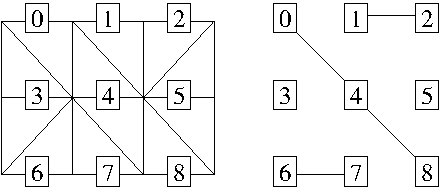
\includegraphics[scale=0.65]{./figuras/laberinto.pdf}
\caption{Grilla con paredes diagonales y el grafo asociado a esta grilla}
\label{fig:laberinto}
\end{figure}

El problema que se quiere resolver es entonces determinar la
cantidad de caminos
simples que empiezan en alguno de los nodos de la
primera fila ($0, 1, ..., m - 1$) y
terminan en alguno de los nodos de la \'ultima fila
($n m, n m + 1, ..., n m + m - 1$).

Los grafos asociados a este tipo de matrices cumplen las siguientes propiedades:

\begin{itemize}
\item Cada nodo tiene grado a lo sumo 2. Esto
es porque un segmento horizontal de la grilla puede
tener a lo sumo un vecino por la celda superior
(como el $0$ respecto del $4$ o la pareja $6$--$7$ en
la Fig.~\ref{fig:laberinto})
y a lo sumo un vecino por la celda inferior (como el $8$ respecto del $4$ o la pareja $1$--$2$). Notar que esto es cierto porque en
{\em todas} las celdas hay una pared.

\item Los nodos de la primera fila y los de la \'ultima
fila tienen grado a lo sumo 1. Los nodos de la primera fila no pueden
tener un vecino por la fila superior, y algo an\'alogo ocurre para los de la \'ultima.

\item Si bien el grafo puede tener ciclos,
no puede haber ciclos alcanzables desde los
nodos de la primera fila. M\'as a\'un, desde
los nodos de la primera fila s\'olo puede
construirse un \'unico camino simple maximal.
Por inducci\'on en la longitud del camino, es
f\'acil ver que todo camino simple
que empiece en un nodo $v_1$ de la primera fila
es o bien $v_1$ (si $v_1$ tiene grado 0)
o bien de la forma
$v_1, ..., v_k$ donde $v_1$ tiene grado 1,
$v_2, ..., v_{k-1}$ tienen grado 2
y $v_k$ tiene grado 1 \'o 2.
Uno de los vecinos de $v_k$ es $v_{k-1}$.
Si $v_k$ tiene grado 1, no tiene m\'as vecinos,
y por lo tanto este es
el \'unico camino simple maximal que se
puede construir a partir de $v_1$.
Si $v_k$ tiene grado 2, tiene un segundo vecino $v_{k+1}$.
Esta es la \'unica manera de extender el camino.
Adem\'as, extendi\'endolo de esta manera
no se forma un ciclo, porque $v_{k+1}$ no puede
ser ninguno de los nodos $v_1, ..., v_{k-1}$
(suponiendo que fuera alguno de dichos nodos, $v_i$,
se concluye que $v_i$ deber\'ia tener grado mayor al
que ya se le conoc\'ia).
\end{itemize}

Teniendo en cuenta la \'ultima propiedad, el algoritmo utilizado
visita cada uno de los nodos de la primera fila y construye
el \'unico camino simple maximal que empieza en ese nodo.
El camino encontrado se considera v\'alido si termina en
alguno de los nodos de la \'ultima fila. Dado que nunca
hay bifurcaciones, no es necesario utilizar una estructura
de datos auxiliar como una pila o una cola
(puede pensarse indistintamente que el algoritmo usado es
DFS o BFS).

Como en cualquier implementaci\'on de BFS, el algoritmo
visita una 'unica vez cada nodo. Para garantizar esto, se mantiene
una estructura (representada con una matriz de booleanos del mismo
tama\~no que la matriz de entrada) en la que se marcan aquellos
nodos que ya fueron visitados.

Dado que los potenciales ciclos del grafo no son alcanzables desde
los nodos asociados a la primera fila de la matriz, el algoritmo
se podr\'ia implementar sin necesidad de mantener esta estructura
auxiliar. Manteni\'endola, se evita recorrer dos veces los caminos
que empiezan y terminan en nodos de la fila superior, lo cual es
potencialmente mejor pero no cambia la complejidad.

El grafo construido tiene $O(n m)$ nodos, y a lo sumo dos ejes
incidentes en cada nodo, de donde resulta que la complejidad del algoritmo
es $O(n m)$, lo cual es lineal en el tama\~no de la entrada.

\subsection{Implementaci�n}
\noindent
\ttfamily
\shorthandoff{"}\\
\hlstd{}\hlline{\ 1\ }\hldir{\#include\ $<$iostream$>$}\\
\hlline{\ 2\ }\hlstd{}\hldir{\#include\ $<$vector$>$}\\
\hlline{\ 3\ }\hlstd{}\hldir{\#include\ $<$cassert$>$}\\
\hlline{\ 4\ }\hlstd{}\hldir{\#include\ $<$cstdio$>$}\\
\hlline{\ 5\ }\hlstd{}\\
\hlline{\ 6\ }\hlkwa{using\ namespace\ }\hlstd{std}\hlsym{;}\\
\hlline{\ 7\ }\hlstd{}\\
\hlline{\ 8\ }\hldir{\#define\ forsn(i,\ s,\ n)\ for\ (int\ i\ =\ (s);\ i\ $<$\ (n);\ i++)}\\
\hlline{\ 9\ }\hlstd{}\hldir{\#define\ forn(i,\ n)\ forsn\ (i,\ 0,\ n)}\\
\hlline{10\ }\hlstd{}\\
\hlline{11\ }\hlkwc{typedef\ }\hlstd{vector}\hlsym{$<$}\hlstd{}\hlkwb{bool}\hlstd{}\hlsym{$>$\ }\hlstd{vbool}\hlsym{;}\\
\hlline{12\ }\hlstd{}\hlkwc{typedef\ }\hlstd{vector}\hlsym{$<$}\hlstd{vbool}\hlsym{$>$\ }\hlstd{vvbool}\hlsym{;}\\
\hlline{13\ }\hlstd{}\\
\hlline{14\ }\hlkwc{typedef\ }\hlstd{}\hlkwb{int\ }\hlstd{Node}\hlsym{;}\\
\hlline{15\ }\hlstd{}\hlkwb{int\ }\hlstd{rows}\hlsym{;}\\
\hlline{16\ }\hlstd{}\hlkwb{int\ }\hlstd{cols}\hlsym{;}\\
\hlline{17\ }\hlstd{vvbool\ mapa}\hlsym{;}\\
\hlline{18\ }\hlstd{}\\
\hlline{19\ }\hldir{\#define\ node(r,\ c)}\hlstd{\ \ }\hldir{((r)\ $<$$<$\ 12\ \textbar \ (c))}\\
\hlline{20\ }\hlstd{}\hldir{\#define\ node\textunderscore row(v)}\hlstd{\ \ }\hldir{((v)\ $>$$>$\ 12)}\\
\hlline{21\ }\hlstd{}\hldir{\#define\ node\textunderscore col(v)}\hlstd{\ \ }\hldir{((v)\ \&\ 0xfff)}\\
\hlline{22\ }\hlstd{}\\
\hlline{23\ }\hldir{\#define\ NONE}\hlstd{\ \ \ }\hldir{0xffffffff}\\
\hlline{24\ }\hlstd{\\
\hlline{25\ }Node\ }\hlkwd{vecino}\hlstd{}\hlsym{(}\hlstd{}\hlkwb{bool\ }\hlstd{ns}\hlsym{,\ }\hlstd{Node\ v}\hlsym{)\ \{}\\
\hlline{26\ }\hlstd{}\hldir{\#define\ sig(x)\ ((x)\ ?\ 1\ :\ {-}1)}\\
\hlline{27\ }\hlstd{\ }\hlkwb{const\ int\ }\hlstd{r\ }\hlsym{=\ }\hlstd{}\hlkwd{node\textunderscore row}\hlstd{}\hlsym{(}\hlstd{v}\hlsym{)\ {-}\ }\hlstd{ns}\hlsym{,\ }\hlstd{c\ }\hlsym{=\ }\hlstd{}\hlkwd{node\textunderscore col}\hlstd{}\hlsym{(}\hlstd{v}\hlsym{);}\\
\hlline{28\ }\hlstd{\ }\hlkwa{if\ }\hlstd{}\hlsym{(}\hlstd{r\ }\hlsym{$<$\ }\hlstd{}\hlnum{0\ }\hlstd{}\hlsym{\textbar \textbar \ }\hlstd{r\ }\hlsym{$>$=\ }\hlstd{rows}\hlsym{)\ }\hlstd{}\hlkwa{return\ }\hlstd{NONE}\hlsym{;}\\
\hlline{29\ }\hlstd{\ }\hlkwb{const\ int\ }\hlstd{cc\ }\hlsym{=\ }\hlstd{c\ }\hlsym{+\ }\hlstd{}\hlkwd{sig}\hlstd{}\hlsym{(}\hlstd{ns\ \textasciicircum \ mapa}\hlsym{{[}}\hlstd{r}\hlsym{{]}{[}}\hlstd{c}\hlsym{{]});}\\
\hlline{30\ }\hlstd{\ }\hlkwa{if\ }\hlstd{}\hlsym{(}\hlstd{cc\ }\hlsym{$<$\ }\hlstd{}\hlnum{0\ }\hlstd{}\hlsym{\textbar \textbar \ }\hlstd{cc\ }\hlsym{$>$=\ }\hlstd{cols}\hlsym{)\ }\hlstd{}\hlkwa{return\ }\hlstd{NONE}\hlsym{;}\\
\hlline{31\ }\hlstd{\ }\hlkwb{const\ int\ }\hlstd{rr\ }\hlsym{=\ }\hlstd{}\hlkwd{node\textunderscore row}\hlstd{}\hlsym{(}\hlstd{v}\hlsym{)\ +\ }\hlstd{}\hlkwd{sig}\hlstd{}\hlsym{(}\hlstd{ns}\hlsym{)\ {*}\ {-}!(}\hlstd{mapa}\hlsym{{[}}\hlstd{r}\hlsym{{]}{[}}\hlstd{c}\hlsym{{]}\ }\hlstd{\textasciicircum \ mapa}\hlsym{{[}}\hlstd{r}\hlsym{{]}{[}}\hlstd{cc}\hlsym{{]});}\\
\hlline{32\ }\hlstd{\ }\hlkwa{if\ }\hlstd{}\hlsym{(}\hlstd{rr\ }\hlsym{$<$\ }\hlstd{}\hlnum{0\ }\hlstd{}\hlsym{\textbar \textbar \ }\hlstd{rr\ }\hlsym{$>$\ }\hlstd{rows}\hlsym{)\ }\hlstd{}\hlkwa{return\ }\hlstd{NONE}\hlsym{;}\\
\hlline{33\ }\hlstd{\ }\hlkwa{return\ }\hlstd{}\hlkwd{node}\hlstd{}\hlsym{(}\hlstd{rr}\hlsym{,\ }\hlstd{cc}\hlsym{);}\\
\hlline{34\ }\hlstd{}\hlsym{\}}\\
\hlline{35\ }\hlstd{}\\
\hlline{36\ }\hlkwb{int\ }\hlstd{}\hlkwd{resolver}\hlstd{}\hlsym{()\ \{}\\
\hlline{37\ }\hlstd{}\hldir{\#define\ marcado(v)\ (\textunderscore marcas{[}node\textunderscore row(v){]}{[}node\textunderscore col(v){]})}\\
\hlline{38\ }\hlstd{}\hldir{\#define\ marcar(v)\ (\textunderscore marcas{[}node\textunderscore row(v){]}{[}node\textunderscore col(v){]}\ =\ true)}\\
\hlline{39\ }\hlstd{\ }\hlkwb{int\ }\hlstd{cant\ }\hlsym{=\ }\hlstd{}\hlnum{0}\hlstd{}\hlsym{;}\\
\hlline{40\ }\hlstd{\ vvbool\ }\hlkwd{\textunderscore marcas}\hlstd{}\hlsym{(}\hlstd{rows\ }\hlsym{+\ }\hlstd{}\hlnum{1}\hlstd{}\hlsym{,\ }\hlstd{}\hlkwd{vbool}\hlstd{}\hlsym{(}\hlstd{cols}\hlsym{,\ }\hlstd{}\hlkwa{false}\hlstd{}\hlsym{));}\\
\hlline{41\ }\hlstd{\ }\hlkwd{forn\ }\hlstd{}\hlsym{(}\hlstd{c}\hlsym{,\ }\hlstd{cols}\hlsym{)\ \{}\\
\hlline{42\ }\hlstd{}\hlstd{\ \ }\hlstd{Node\ v\ }\hlsym{=\ }\hlstd{}\hlkwd{node}\hlstd{}\hlsym{(}\hlstd{}\hlnum{0}\hlstd{}\hlsym{,\ }\hlstd{c}\hlsym{);}\\
\hlline{43\ }\hlstd{\\
\hlline{44\ }}\hlstd{\ \ }\hlstd{}\hlkwa{if\ }\hlstd{}\hlsym{(}\hlstd{}\hlkwd{marcado}\hlstd{}\hlsym{(}\hlstd{v}\hlsym{))\ }\hlstd{}\hlkwa{continue}\hlstd{}\hlsym{;}\\
\hlline{45\ }\hlstd{}\hlstd{\ \ }\hlstd{}\hlkwd{marcar}\hlstd{}\hlsym{(}\hlstd{v}\hlsym{);}\\
\hlline{46\ }\hlstd{\\
\hlline{47\ }}\hlstd{\ \ }\hlstd{}\hlkwa{for\ }\hlstd{}\hlsym{(;;)\ \{}\\
\hlline{48\ }\hlstd{}\hlstd{\ \ \ }\hlstd{Node\ w\ }\hlsym{=\ }\hlstd{NONE}\hlsym{;}\\
\hlline{49\ }\hlstd{}\hlstd{\ \ \ }\hlstd{}\hlkwd{forn\ }\hlstd{}\hlsym{(}\hlstd{direction}\hlsym{,\ }\hlstd{}\hlnum{2}\hlstd{}\hlsym{)\ \{}\\
\hlline{50\ }\hlstd{}\hlstd{\ \ \ \ }\hlstd{Node\ vv\ }\hlsym{=\ }\hlstd{}\hlkwd{vecino}\hlstd{}\hlsym{(}\hlstd{direction}\hlsym{,\ }\hlstd{v}\hlsym{);}\\
\hlline{51\ }\hlstd{}\hlstd{\ \ \ \ }\hlstd{}\hlkwa{if\ }\hlstd{}\hlsym{(}\hlstd{vv\ }\hlsym{==\ }\hlstd{NONE\ }\hlsym{\textbar \textbar \ }\hlstd{}\hlkwd{marcado}\hlstd{}\hlsym{(}\hlstd{vv}\hlsym{))\ }\hlstd{}\hlkwa{continue}\hlstd{}\hlsym{;}\\
\hlline{52\ }\hlstd{}\hlstd{\ \ \ \ }\hlstd{}\hlkwd{assert}\hlstd{}\hlsym{(}\hlstd{w\ }\hlsym{==\ }\hlstd{NONE}\hlsym{);}\\
\hlline{53\ }\hlstd{}\hlstd{\ \ \ \ }\hlstd{w\ }\hlsym{=\ }\hlstd{vv}\hlsym{;}\\
\hlline{54\ }\hlstd{}\hlstd{\ \ \ }\hlstd{}\hlsym{\}}\\
\hlline{55\ }\hlstd{}\hlstd{\ \ \ }\hlstd{}\hlkwa{if\ }\hlstd{}\hlsym{(}\hlstd{w\ }\hlsym{==\ }\hlstd{NONE}\hlsym{)\ }\hlstd{}\hlkwa{break}\hlstd{}\hlsym{;}\\
\hlline{56\ }\hlstd{}\hlstd{\ \ \ }\hlstd{}\hlkwa{if\ }\hlstd{}\hlsym{(}\hlstd{}\hlkwd{node\textunderscore row}\hlstd{}\hlsym{(}\hlstd{w}\hlsym{)\ ==\ }\hlstd{rows}\hlsym{)\ \{}\\
\hlline{57\ }\hlstd{}\hlstd{\ \ \ \ }\hlstd{cant}\hlsym{++;}\\
\hlline{58\ }\hlstd{}\hlstd{\ \ \ \ }\hlstd{}\hlkwa{break}\hlstd{}\hlsym{;}\\
\hlline{59\ }\hlstd{}\hlstd{\ \ \ }\hlstd{}\hlsym{\}}\\
\hlline{60\ }\hlstd{}\hlstd{\ \ \ }\hlstd{}\hlkwd{marcar}\hlstd{}\hlsym{(}\hlstd{w}\hlsym{);}\\
\hlline{61\ }\hlstd{}\hlstd{\ \ \ }\hlstd{v\ }\hlsym{=\ }\hlstd{w}\hlsym{;}\\
\hlline{62\ }\hlstd{}\hlstd{\ \ }\hlstd{}\hlsym{\}}\\
\hlline{63\ }\hlstd{\ }\hlsym{\}}\\
\hlline{64\ }\hlstd{\ }\hlkwa{return\ }\hlstd{cant}\hlsym{;}\\
\hlline{65\ }\hlstd{}\hlsym{\}}\\
\hlline{66\ }\hlstd{}\\
\hlline{67\ }\hlkwb{int\ }\hlstd{}\hlkwd{main}\hlstd{}\hlsym{()\ \{}\\
\hlline{68\ }\hlstd{\ }\hlkwb{int\ }\hlstd{ncases}\hlsym{;}\\
\hlline{69\ }\hlstd{\ cin\ }\hlsym{$>$$>$\ }\hlstd{ncases}\hlsym{;}\\
\hlline{70\ }\hlstd{\ \\
\hlline{71\ }\ }\hlkwd{forn\ }\hlstd{}\hlsym{(}\hlstd{i}\hlsym{,\ }\hlstd{ncases}\hlsym{)\ \{}\\
\hlline{72\ }\hlstd{}\hlstd{\ \ }\hlstd{cin\ }\hlsym{$>$$>$\ }\hlstd{cols\ }\hlsym{$>$$>$\ }\hlstd{rows}\hlsym{;}\\
\hlline{73\ }\hlstd{}\hlstd{\ \ }\hlstd{mapa\ }\hlsym{=\ }\hlstd{}\hlkwd{vvbool}\hlstd{}\hlsym{(}\hlstd{rows}\hlsym{,\ }\hlstd{}\hlkwd{vbool}\hlstd{}\hlsym{(}\hlstd{cols}\hlsym{));}\\
\hlline{74\ }\hlstd{}\hlstd{\ \ }\hlstd{}\hlkwd{forn\ }\hlstd{}\hlsym{(}\hlstd{r}\hlsym{,\ }\hlstd{rows}\hlsym{)\ \{}\\
\hlline{75\ }\hlstd{}\hlstd{\ \ \ }\hlstd{}\hlkwd{forn\ }\hlstd{}\hlsym{(}\hlstd{c}\hlsym{,\ }\hlstd{cols}\hlsym{)\ \{}\\
\hlline{76\ }\hlstd{}\hlstd{\ \ \ \ }\hlstd{}\hlkwb{char\ }\hlstd{mapa\textunderscore rc}\hlsym{;}\\
\hlline{77\ }\hlstd{}\hlstd{\ \ \ \ }\hlstd{cin\ }\hlsym{$>$$>$\ }\hlstd{mapa\textunderscore rc}\hlsym{;}\\
\hlline{78\ }\hlstd{}\hlstd{\ \ \ \ }\hlstd{mapa}\hlsym{{[}}\hlstd{r}\hlsym{{]}{[}}\hlstd{c}\hlsym{{]}\ =\ (}\hlstd{mapa\textunderscore rc\ }\hlsym{==\ }\hlstd{}\hlstr{`}\hlesc{$\backslash$$\backslash$}\hlstr{`}\hlstd{}\hlsym{);}\\
\hlline{79\ }\hlstd{}\hlstd{\ \ \ }\hlstd{}\hlsym{\}}\\
\hlline{80\ }\hlstd{}\hlstd{\ \ }\hlstd{}\hlsym{\}}\\
\hlline{81\ }\hlstd{\\
\hlline{82\ }}\hlstd{\ \ }\hlstd{cout\ }\hlsym{$<$$<$\ }\hlstd{}\hlkwd{resolver}\hlstd{}\hlsym{()\ $<$$<$\ }\hlstd{endl}\hlsym{;}\\
\hlline{83\ }\hlstd{\ }\hlsym{\}}\\
\hlline{84\ }\hlstd{\\
\hlline{85\ }\ }\hlkwa{return\ }\hlstd{}\hlnum{0}\hlstd{}\hlsym{;}\\
\hlline{86\ }\hlstd{}\hlsym{\}}\hlstd{}\\
\mbox{}
\normalfont
\shorthandon{"}




\label{LastPage}
\end{document}

